% E-Portfolio Tempalate for Christ University - School of Engineering and Technology
% Developer: Dr Venkataswamy R, Associate Professor, EEE
% https://github.com/venkataswamyr
% Release Date: 15 November 2025
% Mentor: Dr Raghunandan Kumar, Dean, SoET, Christ University

\documentclass[final,20pt,a4paper]{beamer}

% ====================
% Packages
% ====================

\usepackage{lmodern}
\usepackage{beamerposter}
\usetheme{gemini}
\usecolortheme{gemini}
\usepackage{graphicx}
\usepackage{booktabs}
\usepackage{tikz}
\usepackage{pgfplots}
\pgfplotsset{compat=1.18}
\usepackage{anyfontsize}
\usepackage{xifthen}
\usepackage{calc}
\usepackage{array}
\usepackage{graphicx}
\usepackage{wrapfig}
\usepackage{color}
\usepackage{fontawesome5}
\usepackage{booktabs}
\usepackage{colortbl}
\usepackage{xcolor}


% E-Portfolio Tempalate for Christ University - School of Engineering and Technology
% Developer: Dr Venkataswamy R, Associate Professor, EEE
% https://github.com/venkataswamyr
% Release Date: 15 November 2025
% Mentor: Dr Raghunandan Kumar, Dean, SoET, Christ University

\newcommand{\UniversityName}
{CHRIST (Deemed to be University)}

\newcommand{\CollegeName}
{School of Engineering and Technology}

\newcommand{\StudentName}
{Venkataswamy Ramu}

\newcommand{\StudentRegNo}
{1234567}

\newcommand{\StudentPhoto}
{images/Venkat.jpg}

\newcommand{\StudentDepartment}
{Department of Electrical and Electronics Engineering}

\newcommand{\AcademicYear}
{2024-2025}

\newcommand{\GoalOne}
{To establish a startup company in generative AI that focuses on developing innovative AI-driven solutions for content creation and automation.}

\newcommand{\GoalTwo}
{To get admission in top 10 universities for a Master's program in Computer Science by achieving a GRE score of 320+ and a TOEFL score of 100+.}

\newcommand{\GoalThree}
{To get job offer from a leading semiconductor company by completing relevant internships and projects in the field of VLSI design and embedded systems.}

\newcommand{\PGYear}
{2025}

\newcommand{\PGSpecialization}
{Electric Vehicle Technology}

\newcommand{\PGCGPA}
{4.75}

\newcommand{\PGCGPAMax}
{5.00}

\newcommand{\PGStatus}
{Ongoing}

\newcommand{\UGYear}
{2023}

\newcommand{\UGSpecialization}
{Electrical and Electronics Engineering}

\newcommand{\UGCGPA}
{4.75}

\newcommand{\UGCGPAMax}
{5.00}

\newcommand{\UGStatus}
{Completed}

\newcommand{\PUCYear}
{2019}

\newcommand{\PUCSpecialization}
{PCMC}

\newcommand{\PUCCollege}
{JSS PU College}

\newcommand{\PUCMarks}
{89}

\newcommand{\PUCMarksMax}
{100}

\newcommand{\PUCStatus}
{Completed}


\newcommand{\MetriculationYear}
{2017}

\newcommand{\MetriculationBoard}
{CBSE}

\newcommand{\MetriculationSchool}
{Christ School}

\newcommand{\MetriculationMarks}
{89}

\newcommand{\MetriculationMarksMax}
{100}

\newcommand{\MetriculationStatus}
{Completed}

\newcommand{\DiplomaYear}
{}

\newcommand{\DiplomaSpecilization}
{Fitter}

\newcommand{\DiplomaCollege}
{Christ School}

\newcommand{\DiplomaMarks}
{89}

\newcommand{\DiplomaMarksMax}
{100}

\newcommand{\DiplomaStatus}
{Completed}


\newcommand{\LinkedInURL}
{https://www.linkedin.com/in/venkataswamy-r-1234567/}

\newcommand{\GithubURL}
{https://github.com/yourusername}

\newcommand{\TwitterURL}
{https://twitter.com/yourusername}

\newcommand{\PortfolioURL}
{https://yourportfolio.com}

\newcommand{\OrcidURL}
{https://orcid.org}

\newcommand{\GoogleScholarURL}
{https://scholar.google.com/citations?user=yourid}

\newcommand{\EmailID}
{venkataswamy.r@christuniversity.in}

\newcommand{\MobileNo}
{+917829222446}

\newcommand{\AreaOfInterestOne}
{E-Mobility}

\newcommand{\AreaOfInterestTwo}
{Artificial Intelligence}

\newcommand{\AreaOfInterestThree}
{Aerospace Systems}

\newcommand{\TechnologyToolOne}
{Autocad Electrical}

\newcommand{\TechnologyToolOneValue}
{7}

\newcommand{\TechnologyToolTwo}
{Matlab Simulink}

\newcommand{\TechnologyToolTwoValue}
{3}

\newcommand{\TechnologyToolThree}
{Matlab Simulink}

\newcommand{\TechnologyToolThreeValue}
{3}

\newcommand{\TechnologyToolFour}
{Matlab Simulink}

\newcommand{\TechnologyToolFourValue}
{3}

\newcommand{\TechnologyToolFive}
{Matlab Simulink}

\newcommand{\TechnologyToolFiveValue}
{3}

\newcommand{\TechnologyToolSix}
{Matlab Simulink}

\newcommand{\TechnologyToolSixValue}
{3}

\newcommand{\TechnologyToolSeven}
{Matlab Simulink}

\newcommand{\TechnologyToolSevenValue}
{3}

\newcommand{\TechnologyToolEight}
{Matlab Simulink}

\newcommand{\TechnologyToolEightValue}
{3}


\newcommand{\SkillOne}
{Python Programming}

\newcommand{\SkillOneValue}
{3.2}

\newcommand{\SkillTwo}
{Generative AI}

\newcommand{\SkillTwoValue}
{2}

\newcommand{\SkillThree}
{Cloud Computing}

\newcommand{\SkillThreeValue}
{2}

\newcommand{\SkillFour}
{Digital Twin}

\newcommand{\SkillFourValue}
{2}

\newcommand{\AchievmentRoleResponsibility}
{IEEE CIS Chair & IEEE event organization, Team mangement\\
CSA Member  & Involved in Social activities\\
EETA Secretory  & Conducted sports and cultural events \\
Hackathon Winner & Developed innovative solutions under time constraints \\
}

% Project 1

\newcommand{\ProjectTitleOne}
{Internet of Things Enabled Digital Twin of Patient in Healthcare and Predictive Analysis using Machine Leaning}
\newcommand{\ProjectDescriptionOne}
{Internet of Things, artificial intelligence, and digital twin technologies are employed to improve patient care, overall efficiency of the healthcare system, and realistic experience with reduced operational costs.}
\newcommand{\ProjectImageFirstOne}
{images/dt1.png}
\newcommand{\ProjectImageFirstCaptionOne}
{Digital Twin of Healthcare Person}
\newcommand{\ProjectImageFirstScaleOne}
{1.1}
\newcommand{\ProjectImageSecondOne}
{images/system22.png}
\newcommand{\ProjectImageSecondCaptionOne}
{Block Diagram of Digital Twin System}  
\newcommand{\ProjectImageSecondScaleOne}
{2.4}
\newcommand{\ProjectOutcomeOne}
{Patient data extracted to digital twin.}

% Project 2

\newcommand{\ProjectTitleTwo}
{Internet of Things Enabled Digital Twin of Patient in Healthcare and Predictive Analysis using Machine Leaning}
\newcommand{\ProjectDescriptionTwo}
{Internet of Things, artificial intelligence, and digital twin technologies are employed to improve patient care, overall efficiency of the healthcare system, and realistic experience with reduced operational costs.}
\newcommand{\ProjectImageFirstTwo}
{images/dt1.png}
\newcommand{\ProjectImageFirstCaptionTwo}
{Digital Twin of Healthcare Person}
\newcommand{\ProjectImageFirstScaleTwo}
{1.1}
\newcommand{\ProjectImageSecondTwo}
{images/system22.png}
\newcommand{\ProjectImageSecondCaptionTwo}
{Block Diagram of Digital Twin System}  
\newcommand{\ProjectImageSecondScaleTwo}
{2.4}
\newcommand{\ProjectOutcomeTwo}
{Patient data extracted to digital twin.}

% Project 3
\newcommand{\ProjectTitleThree}
{}
\newcommand{\ProjectDescriptionThree}
{}
\newcommand{\ProjectImageFirstThree}
{}
\newcommand{\ProjectImageFirstCaptionThree}
{}
\newcommand{\ProjectImageFirstScaleThree}
{}
\newcommand{\ProjectImageSecondThree}
{}
\newcommand{\ProjectImageSecondCaptionThree}
{}  
\newcommand{\ProjectImageSecondScaleThree}
{}
\newcommand{\ProjectOutcomeThree}
{}

% Project 4
\newcommand{\ProjectTitleFour}
{}
\newcommand{\ProjectDescriptionFour}
{}
\newcommand{\ProjectImageFirstFour}
{}
\newcommand{\ProjectImageFirstCaptionFour}
{}
\newcommand{\ProjectImageFirstScaleFour}
{}
\newcommand{\ProjectImageSecondFour}
{}
\newcommand{\ProjectImageSecondCaptionFour}
{}  
\newcommand{\ProjectImageSecondScaleFour}
{}
\newcommand{\ProjectOutcomeFour}
{}


% Project 5
\newcommand{\ProjectTitleFive}
{}
\newcommand{\ProjectDescriptionFive}
{}
\newcommand{\ProjectImageFirstFive}
{}
\newcommand{\ProjectImageFirstCaptionFive}
{}
\newcommand{\ProjectImageFirstScaleFive}
{}
\newcommand{\ProjectImageSecondFive}
{}
\newcommand{\ProjectImageSecondCaptionFive}
{}  
\newcommand{\ProjectImageSecondScaleFive}
{}
\newcommand{\ProjectOutcomeFive}
{}

% Project 6
\newcommand{\ProjectTitleSix}
{}
\newcommand{\ProjectDescriptionSix}
{}
\newcommand{\ProjectImageFirstSix}
{}
\newcommand{\ProjectImageFirstCaptionSix}
{}
\newcommand{\ProjectImageFirstScaleSix}
{}
\newcommand{\ProjectImageSecondSix}
{}
\newcommand{\ProjectImageSecondCaptionSix}
{}  
\newcommand{\ProjectImageSecondScaleSix}
{}
\newcommand{\ProjectOutcomeSix}
{}

% Project 7
\newcommand{\ProjectTitleSeven}
{}
\newcommand{\ProjectDescriptionSeven}
{}
\newcommand{\ProjectImageFirstSeven}
{}
\newcommand{\ProjectImageFirstCaptionSeven}
{}
\newcommand{\ProjectImageFirstScaleSeven}
{}
\newcommand{\ProjectImageSecondSeven}
{}
\newcommand{\ProjectImageSecondCaptionSeven}
{}  
\newcommand{\ProjectImageSecondScaleSeven}
{}
\newcommand{\ProjectOutcomeSeven}
{}

% Project 8
\newcommand{\ProjectTitleEight}
{}
\newcommand{\ProjectDescriptionEight}
{}
\newcommand{\ProjectImageFirstEight}
{}
\newcommand{\ProjectImageFirstCaptionEight}
{}
\newcommand{\ProjectImageFirstScaleEight}
{}
\newcommand{\ProjectImageSecondEight}
{}
\newcommand{\ProjectImageSecondCaptionEight}
{}  
\newcommand{\ProjectImageSecondScaleEight}
{}
\newcommand{\ProjectOutcomeEight}
{}

% Project 9
\newcommand{\ProjectTitleNine}
{}
\newcommand{\ProjectDescriptionNine}
{}
\newcommand{\ProjectImageFirstNine}
{}
\newcommand{\ProjectImageFirstCaptionNine}
{}
\newcommand{\ProjectImageFirstScaleNine}
{}
\newcommand{\ProjectImageSecondNine}
{}
\newcommand{\ProjectImageSecondCaptionNine}
{}  
\newcommand{\ProjectImageSecondScaleNine}
{}
\newcommand{\ProjectOutcomeNine}
{}

% Project 10
\newcommand{\ProjectTitleTen}
{}
\newcommand{\ProjectDescriptionTen}
{}
\newcommand{\ProjectImageFirstTen}
{}
\newcommand{\ProjectImageFirstCaptionTen}
{}
\newcommand{\ProjectImageFirstScaleTen}
{}
\newcommand{\ProjectImageSecondTen}
{}
\newcommand{\ProjectImageSecondCaptionTen}
{}  
\newcommand{\ProjectImageSecondScaleTen}
{}
\newcommand{\ProjectOutcomeTen}
{}



% Research 1
\newcommand{\ResearchTitleOne}
{Novel System Indicators for Diagnostics of Winding}
\newcommand{\ResearchDescriptionOne}
{System indicators are proposed for the characterization of frequency response of a transformer winding. Axial and radial  deformations of the transformer winding are identified}
\newcommand{\ResearchImageFirstOne}
{images/tran2.eps}
\newcommand{\ResearchImageFirstCaptionOne}
{System Indicators for Transformer Winding}
\newcommand{\ResearchImageFirstScaleOne}
{2}
\newcommand{\ResearchImageSecondOne}
{images/tran1.eps}
\newcommand{\ResearchImageSecondCaptionOne}
{Comparision of Frequency Response}  
\newcommand{\ResearchImageSecondScaleOne}
{1}
\newcommand{\ResearchOutcomeOne}
{Fault location and extent are identified.}

% Research 2
\newcommand{\ResearchTitleTwo}
{}
\newcommand{\ResearchDescriptionTwo}
{}
\newcommand{\ResearchImageFirstTwo}
{}
\newcommand{\ResearchImageFirstCaptionTwo}
{}
\newcommand{\ResearchImageFirstScaleTwo}
{}
\newcommand{\ResearchImageSecondTwo}
{}
\newcommand{\ResearchImageSecondCaptionTwo}
{}  
\newcommand{\ResearchImageSecondScaleTwo}
{}
\newcommand{\ResearchOutcomeTwo}
{}

% Research 3
\newcommand{\ResearchTitleThree}
{}
\newcommand{\ResearchDescriptionThree}
{}
\newcommand{\ResearchImageFirstThree}
{}
\newcommand{\ResearchImageFirstCaptionThree}
{}
\newcommand{\ResearchImageFirstScaleThree}
{}
\newcommand{\ResearchImageSecondThree}
{}
\newcommand{\ResearchImageSecondCaptionThree}
{}  
\newcommand{\ResearchImageSecondScaleThree}
{}
\newcommand{\ResearchOutcomeThree}
{}

% Research 4
\newcommand{\ResearchTitleFour}
{}
\newcommand{\ResearchDescriptionFour}
{}
\newcommand{\ResearchImageFirstFour}
{}
\newcommand{\ResearchImageFirstCaptionFour}
{}
\newcommand{\ResearchImageFirstScaleFour}
{}
\newcommand{\ResearchImageSecondFour}
{}
\newcommand{\ResearchImageSecondCaptionFour}
{}  
\newcommand{\ResearchImageSecondScaleFour}
{}
\newcommand{\ResearchOutcomeFour}
{}

% Research 5
\newcommand{\ResearchTitleFive}
{}
\newcommand{\ResearchDescriptionFive}
{}
\newcommand{\ResearchImageFirstFive}
{}
\newcommand{\ResearchImageFirstCaptionFive}
{}
\newcommand{\ResearchImageFirstScaleFive}
{}
\newcommand{\ResearchImageSecondFive}
{}
\newcommand{\ResearchImageSecondCaptionFive}
{}  
\newcommand{\ResearchImageSecondScaleFive}
{}
\newcommand{\ResearchOutcomeFive}
{}

% Research 6
\newcommand{\ResearchTitleSix}
{}
\newcommand{\ResearchDescriptionSix}
{}
\newcommand{\ResearchImageFirstSix}
{}
\newcommand{\ResearchImageFirstCaptionSix}
{}
\newcommand{\ResearchImageFirstScaleSix}
{}
\newcommand{\ResearchImageSecondSix}
{}
\newcommand{\ResearchImageSecondCaptionSix}
{}  
\newcommand{\ResearchImageSecondScaleSix}
{}
\newcommand{\ResearchOutcomeSix}
{}

% Research 7
\newcommand{\ResearchTitleSeven}
{}
\newcommand{\ResearchDescriptionSeven}
{}
\newcommand{\ResearchImageFirstSeven}
{}
\newcommand{\ResearchImageFirstCaptionSeven}
{}
\newcommand{\ResearchImageFirstScaleSeven}
{}
\newcommand{\ResearchImageSecondSeven}
{}
\newcommand{\ResearchImageSecondCaptionSeven}
{}  
\newcommand{\ResearchImageSecondScaleSeven}
{}
\newcommand{\ResearchOutcomeSeven}
{}

% Research 8
\newcommand{\ResearchTitleEight}
{}
\newcommand{\ResearchDescriptionEight}
{}
\newcommand{\ResearchImageFirstEight}
{}
\newcommand{\ResearchImageFirstCaptionEight}
{}
\newcommand{\ResearchImageFirstScaleEight}
{}
\newcommand{\ResearchImageSecondEight}
{}
\newcommand{\ResearchImageSecondCaptionEight}
{}  
\newcommand{\ResearchImageSecondScaleEight}
{}
\newcommand{\ResearchOutcomeEight}
{}

% Research 9
\newcommand{\ResearchTitleNine}
{}
\newcommand{\ResearchDescriptionNine}
{}
\newcommand{\ResearchImageFirstNine}
{}
\newcommand{\ResearchImageFirstCaptionNine}
{}
\newcommand{\ResearchImageFirstScaleNine}
{}
\newcommand{\ResearchImageSecondNine}
{}
\newcommand{\ResearchImageSecondCaptionNine}
{}  
\newcommand{\ResearchImageSecondScaleNine}
{}
\newcommand{\ResearchOutcomeNine}
{}

% Research 10
\newcommand{\ResearchTitleTen}
{}
\newcommand{\ResearchDescriptionTen}
{}
\newcommand{\ResearchImageFirstTen}
{}
\newcommand{\ResearchImageFirstCaptionTen}
{}
\newcommand{\ResearchImageFirstScaleTen}
{}
\newcommand{\ResearchImageSecondTen}
{}
\newcommand{\ResearchImageSecondCaptionTen}
{}  
\newcommand{\ResearchImageSecondScaleTen}
{}
\newcommand{\ResearchOutcomeTen}
{}


% Activity 1
\newcommand{\ActivityTitleOne}
{IEEE BC}
\newcommand{\ActivityDescriptionOne}
{Excited to be a part of IEEE India Blockchain Forum. Hosted by Dept of EEE, Christ University}
\newcommand{\ActivityImageFirstOne}
{images/pic2.jpg}
\newcommand{\ActivityImageFirstCaptionOne}
{Event}
\newcommand{\ActivityImageFirstScaleOne}
{0.4}
\newcommand{\ActivityImageSecondOne}
{images/pic2.jpg}
\newcommand{\ActivityImageSecondCaptionOne}
{Event}  
\newcommand{\ActivityImageSecondScaleOne}
{0.4}
\newcommand{\ActivityOutcomeOne}
{Learn Leadership Skill}

% Activity 2
\newcommand{\ActivityTitleTwo}
{}
\newcommand{\ActivityDescriptionTwo}
{}
\newcommand{\ActivityImageFirstTwo}
{}
\newcommand{\ActivityImageFirstCaptionTwo}
{}
\newcommand{\ActivityImageFirstScaleTwo}
{}
\newcommand{\ActivityImageSecondTwo}
{}
\newcommand{\ActivityImageSecondCaptionTwo}
{}  
\newcommand{\ActivityImageSecondScaleTwo}
{}
\newcommand{\ActivityOutcomeTwo}
{}

% Activity 3
\newcommand{\ActivityTitleThree}
{}
\newcommand{\ActivityDescriptionThree}
{}
\newcommand{\ActivityImageFirstThree}
{}
\newcommand{\ActivityImageFirstCaptionThree}
{}
\newcommand{\ActivityImageFirstScaleThree}
{}
\newcommand{\ActivityImageSecondThree}
{}
\newcommand{\ActivityImageSecondCaptionThree}
{}  
\newcommand{\ActivityImageSecondScaleThree}
{}
\newcommand{\ActivityOutcomeThree}
{}

% Activity 4
\newcommand{\ActivityTitleFour}
{}
\newcommand{\ActivityDescriptionFour}
{}
\newcommand{\ActivityImageFirstFour}
{}
\newcommand{\ActivityImageFirstCaptionFour}
{}
\newcommand{\ActivityImageFirstScaleFour}
{}
\newcommand{\ActivityImageSecondFour}
{}
\newcommand{\ActivityImageSecondCaptionFour}
{}  
\newcommand{\ActivityImageSecondScaleFour}
{}
\newcommand{\ActivityOutcomeFour}
{}

% Activity 5
\newcommand{\ActivityTitleFive}
{}
\newcommand{\ActivityDescriptionFive}
{}
\newcommand{\ActivityImageFirstFive}
{}
\newcommand{\ActivityImageFirstCaptionFive}
{}
\newcommand{\ActivityImageFirstScaleFive}
{}
\newcommand{\ActivityImageSecondFive}
{}
\newcommand{\ActivityImageSecondCaptionFive}
{}  
\newcommand{\ActivityImageSecondScaleFive}
{}
\newcommand{\ActivityOutcomeFive}
{}

% Activity 6
\newcommand{\ActivityTitleSix}
{}
\newcommand{\ActivityDescriptionSix}
{}
\newcommand{\ActivityImageFirstSix}
{}
\newcommand{\ActivityImageFirstCaptionSix}
{}
\newcommand{\ActivityImageFirstScaleSix}
{}
\newcommand{\ActivityImageSecondSix}
{}
\newcommand{\ActivityImageSecondCaptionSix}
{}  
\newcommand{\ActivityImageSecondScaleSix}
{}
\newcommand{\ActivityOutcomeSix}
{}

% Activity 7
\newcommand{\ActivityTitleSeven}
{}
\newcommand{\ActivityDescriptionSeven}
{}
\newcommand{\ActivityImageFirstSeven}
{}
\newcommand{\ActivityImageFirstCaptionSeven}
{}
\newcommand{\ActivityImageFirstScaleSeven}
{}
\newcommand{\ActivityImageSecondSeven}
{}
\newcommand{\ActivityImageSecondCaptionSeven}
{}  
\newcommand{\ActivityImageSecondScaleSeven}
{}
\newcommand{\ActivityOutcomeSeven}
{}

% Activity 8
\newcommand{\ActivityTitleEight}
{}
\newcommand{\ActivityDescriptionEight}
{}
\newcommand{\ActivityImageFirstEight}
{}
\newcommand{\ActivityImageFirstCaptionEight}
{}
\newcommand{\ActivityImageFirstScaleEight}
{}
\newcommand{\ActivityImageSecondEight}
{}
\newcommand{\ActivityImageSecondCaptionEight}
{}  
\newcommand{\ActivityImageSecondScaleEight}
{}
\newcommand{\ActivityOutcomeEight}
{}

% Activity 9
\newcommand{\ActivityTitleNine}
{}
\newcommand{\ActivityDescriptionNine}
{}
\newcommand{\ActivityImageFirstNine}
{}
\newcommand{\ActivityImageFirstCaptionNine}
{}
\newcommand{\ActivityImageFirstScaleNine}
{}
\newcommand{\ActivityImageSecondNine}
{}
\newcommand{\ActivityImageSecondCaptionNine}
{}  
\newcommand{\ActivityImageSecondScaleNine}
{}
\newcommand{\ActivityOutcomeNine}
{}

% Activity 10
\newcommand{\ActivityTitleTen}
{}
\newcommand{\ActivityDescriptionTen}
{}
\newcommand{\ActivityImageFirstTen}
{}
\newcommand{\ActivityImageFirstCaptionTen}
{}
\newcommand{\ActivityImageFirstScaleTen}
{}
\newcommand{\ActivityImageSecondTen}
{}
\newcommand{\ActivityImageSecondCaptionTen}
{}  
\newcommand{\ActivityImageSecondScaleTen}
{}
\newcommand{\ActivityOutcomeTen}
{}

% Activity 11
\newcommand{\ActivityTitleEleven}
{}
\newcommand{\ActivityDescriptionEleven}
{}
\newcommand{\ActivityImageFirstEleven}
{}
\newcommand{\ActivityImageFirstCaptionEleven}
{}
\newcommand{\ActivityImageFirstScaleEleven}
{}
\newcommand{\ActivityImageSecondEleven}
{}
\newcommand{\ActivityImageSecondCaptionEleven}
{}  
\newcommand{\ActivityImageSecondScaleEleven}
{}
\newcommand{\ActivityOutcomeEleven}
{}

% Activity 12
\newcommand{\ActivityTitleTwelve}
{}
\newcommand{\ActivityDescriptionTwelve}
{}
\newcommand{\ActivityImageFirstTwelve}
{}
\newcommand{\ActivityImageFirstCaptionTwelve}
{}
\newcommand{\ActivityImageFirstScaleTwelve}
{}
\newcommand{\ActivityImageSecondTwelve}
{}
\newcommand{\ActivityImageSecondCaptionTwelve}
{}  
\newcommand{\ActivityImageSecondScaleTwelve}
{}
\newcommand{\ActivityOutcomeTwelve}
{}

% Activity 13
\newcommand{\ActivityTitleThirteen}
{}
\newcommand{\ActivityDescriptionThirteen}
{}
\newcommand{\ActivityImageFirstThirteen}
{}
\newcommand{\ActivityImageFirstCaptionThirteen}
{}
\newcommand{\ActivityImageFirstScaleThirteen}
{}
\newcommand{\ActivityImageSecondThirteen}
{}
\newcommand{\ActivityImageSecondCaptionThirteen}
{}  
\newcommand{\ActivityImageSecondScaleThirteen}
{}
\newcommand{\ActivityOutcomeThirteen}
{}

% Activity 14
\newcommand{\ActivityTitleFourteen}
{}
\newcommand{\ActivityDescriptionFourteen}
{}
\newcommand{\ActivityImageFirstFourteen}
{}
\newcommand{\ActivityImageFirstCaptionFourteen}
{}
\newcommand{\ActivityImageFirstScaleFourteen}
{}
\newcommand{\ActivityImageSecondFourteen}
{}
\newcommand{\ActivityImageSecondCaptionFourteen}
{}  
\newcommand{\ActivityImageSecondScaleFourteen}
{}
\newcommand{\ActivityOutcomeFourteen}
{}

% Activity 15
\newcommand{\ActivityTitleFifteen}
{}
\newcommand{\ActivityDescriptionFifteen}
{}
\newcommand{\ActivityImageFirstFifteen}
{}
\newcommand{\ActivityImageFirstCaptionFifteen}
{}
\newcommand{\ActivityImageFirstScaleFifteen}
{}
\newcommand{\ActivityImageSecondFifteen}
{}
\newcommand{\ActivityImageSecondCaptionFifteen}
{}  
\newcommand{\ActivityImageSecondScaleFifteen}
{}
\newcommand{\ActivityOutcomeFifteen}
{}

% Activity 16
\newcommand{\ActivityTitleSixteen}
{}
\newcommand{\ActivityDescriptionSixteen}
{}
\newcommand{\ActivityImageFirstSixteen}
{}
\newcommand{\ActivityImageFirstCaptionSixteen}
{}
\newcommand{\ActivityImageFirstScaleSixteen}
{}
\newcommand{\ActivityImageSecondSixteen}
{}
\newcommand{\ActivityImageSecondCaptionSixteen}
{}  
\newcommand{\ActivityImageSecondScaleSixteen}
{}
\newcommand{\ActivityOutcomeSixteen}
{}

% Activity 17
\newcommand{\ActivityTitleSeventeen}
{}
\newcommand{\ActivityDescriptionSeventeen}
{}
\newcommand{\ActivityImageFirstSeventeen}
{}
\newcommand{\ActivityImageFirstCaptionSeventeen}
{}
\newcommand{\ActivityImageFirstScaleSeventeen}
{}
\newcommand{\ActivityImageSecondSeventeen}
{}
\newcommand{\ActivityImageSecondCaptionSeventeen}
{}  
\newcommand{\ActivityImageSecondScaleSeventeen}
{}
\newcommand{\ActivityOutcomeSeventeen}
{}

% Activity 18
\newcommand{\ActivityTitleEighteen}
{}
\newcommand{\ActivityDescriptionEighteen}
{}
\newcommand{\ActivityImageFirstEighteen}
{}
\newcommand{\ActivityImageFirstCaptionEighteen}
{}
\newcommand{\ActivityImageFirstScaleEighteen}
{}
\newcommand{\ActivityImageSecondEighteen}
{}
\newcommand{\ActivityImageSecondCaptionEighteen}
{}  
\newcommand{\ActivityImageSecondScaleEighteen}
{}
\newcommand{\ActivityOutcomeEighteen}
{}

% Activity 19
\newcommand{\ActivityTitleNineteen}
{}
\newcommand{\ActivityDescriptionNineteen}
{}
\newcommand{\ActivityImageFirstNineteen}
{}
\newcommand{\ActivityImageFirstCaptionNineteen}
{}
\newcommand{\ActivityImageFirstScaleNineteen}
{}
\newcommand{\ActivityImageSecondNineteen}
{}
\newcommand{\ActivityImageSecondCaptionNineteen}
{}  
\newcommand{\ActivityImageSecondScaleNineteen}
{}
\newcommand{\ActivityOutcomeNineteen}
{}

% Activity 20
\newcommand{\ActivityTitleTwenty}
{}
\newcommand{\ActivityDescriptionTwenty}
{}
\newcommand{\ActivityImageFirstTwenty}
{}
\newcommand{\ActivityImageFirstCaptionTwenty}
{}
\newcommand{\ActivityImageFirstScaleTwenty}
{}
\newcommand{\ActivityImageSecondTwenty}
{}
\newcommand{\ActivityImageSecondCaptionTwenty}
{}  
\newcommand{\ActivityImageSecondScaleTwenty}
{}
\newcommand{\ActivityOutcomeTwenty}
{}



% ====================
% Lengths
% ====================

% If you have N columns, choose \sepwidth and \colwidth such that
% (N+1)*\sepwidth + N*\colwidth = \paperwidth
\newlength{\sepwidth}
\newlength{\colwidth}
\setlength{\sepwidth}{0.025\paperwidth}
\setlength{\colwidth}{0.465\paperwidth}

\newcommand{\separatorcolumn}{\begin{column}{\sepwidth}\end{column}}
\title{{\fontsize{80}{40}\selectfont \StudentName}}
\author{\huge{E-PORTFOLIO}}

% Define watermark
\setbeamertemplate{background}{%
    \begin{tikzpicture}[remember picture, overlay]
        \node[opacity=0.2] at (current page.center) 
            {\includegraphics[width=0.3\paperwidth]{assets/logoback.png}};
    \end{tikzpicture}%
}

\footercontent{
  \href{https://www.christuniversity.in}{https://www.christuniversity.in} \hfill
\huge{
\href{\LinkedInURL}{\textcolor{white!80!black}{\faLinkedin}}\hspace{1cm}
\href{\GithubURL}{\textcolor{white}{\faGithub}} \hspace{1cm}
\href{\TwitterURL}{\textcolor{white!50}{\faTwitter}} \hspace{1cm}
\href{\PortfolioURL}{\textcolor{white}{\faGlobe}}
}
 \hfill
  \href{https://christuniversity.in/schools/school-of-engineering-and-technology}{\CollegeName}}


% use this to include logos on the left and/or right side of the header:
\logoright{\includegraphics[height=7cm]{assets/logo1.png}}
\logoleft{\includegraphics[height=7cm]{\StudentPhoto}}

% custom column width
\newcolumntype{x}[1]{%
>{\raggedleft\hspace{0pt}}p{#1}}%

\usetikzlibrary{shapes, backgrounds}

\newcommand{\vcenteredinclude}[1]{\begingroup
\setbox0=\hbox{\includegraphics{#1}}%
\parbox{\wd0}{\box0}\endgroup}

\newcommand*{\vcenteredhbox}[1]{\begingroup
\setbox0=\hbox{#1}\parbox{\wd0}{\box0}\endgroup}


\definecolor{maincol}{RGB}{255,150,0}

%secondary colors
\definecolor{secondcol}{RGB}{0,178,255}
\definecolor{thirdcol}{RGB}{0,80,130}
\definecolor{fourthcol}{RGB}{0,100,160}
\definecolor{fifthcol}{RGB}{0,120,200}
\definecolor{sixthcol}{RGB}{0,80,130}

%background color
\definecolor{bgcol}{RGB}{190,220,255}

%textcolor
\definecolor{textcol}{RGB}{0,50,80}

%sectioncolor
\definecolor{sectcol}{RGB}{255,255,255}

%set a background col for whole page
\pagecolor{bgcol}

% a six pointed arrow poiting to the left
\newcommand{\tzlarrow}{(0,0) -- (0.2,0) -- (0.3,0.2) -- (0.2,0.4) -- (0,0.4) -- (0.1,0.2) -- cycle;}	

% a six pointed arrow poiting to the right
\newcommand{\tzrarrow}{ (0,0.2) -- (0.1,0) -- (0.3,0) -- (0.2,0.2) -- (0.3,0.4) -- (0.1,0.4) -- cycle;}


% include the left arrow into a tikz picture
% param1: fill color
%
\newcommand{\larrow}[1]
{\begin{tikzpicture}[scale=0.58]
	 \filldraw[fill=#1!100,draw=#1!100!black]  \tzlarrow
 \end{tikzpicture}
}

% include the right arrow into a tikz picture
% param1: fill color
%
\newcommand{\rarrow}[1]
{\begin{tikzpicture}[scale=0.58]
	\filldraw[fill=#1!100,draw=#1!100!black] \tzrarrow
 \end{tikzpicture}
}

% the chart graphics are outsourced into own files

%----------------------------------------------------------------------------------------
% 	PIE CHART
%----------------------------------------------------------------------------------------
\input{assets/chart/chart.tex}

%----------------------------------------------------------------------------------------
% 	BAR CHART
%----------------------------------------------------------------------------------------
\input{assets/chart/barchart.tex}

%----------------------------------------------------------------------------------------
% 	BUBBLE CHART
%----------------------------------------------------------------------------------------
\input{assets/chart/bubbles.tex}

%----------------------------------------------------------------------------------------
% 	TIMELINE CHART
%----------------------------------------------------------------------------------------
\input{assets/chart/timeline.tex}

%----------------------------------------------------------------------------------------
% 	FACT BUBBLE
%----------------------------------------------------------------------------------------
\input{assets/chart/factbubble.tex}


\newcommand{\cvsection}[2] {
\textcolor{sectcol}{\uppercase{\textbf{#1}}}
}

\newcommand{\cvsect}[4]{
	\textcolor{#3}{\hrule}
	\colorbox{#3}{ {\cvsection{#1}{#4}}}
}

% create a coloured arrow with title as cv meta section section
% param 1: meta section title
%
\newcommand{\metasection}[2] {
	\begin{tabular*}{1\textwidth}{ l l }
		#1&#2\\[12pt]
	\end{tabular*}
}

% creates a stretched box as 
\newcommand{\cveventmeta}[2] {
	\mbox{\mystrut \hspace{87pt}\textit{#1}}\\
	#2
}


% custom strut
\newcommand{\mystrut}{\rule[-.3\baselineskip]{0pt}{\baselineskip}}

% colored rule and text for chart legends, wrapped in parbox
% param 1: text
% param 2: width in cm or pt, em ...
% param 3: color
\newcommand{\legend}[3]{\parbox{#2}{\textcolor{#3}{\rule{#2}{4pt}}\\#1}}

%----------------------------------------------------------------------------------------
% CUSTOM LOREM IPSUM
%----------------------------------------------------------------------------------------
\newcommand{\lorem}{Lorem ipsum dolor sit amet, consectetur adipiscing elit. Donec a diam lectus.}

\newcommand{\varitem}[3][black]{%
  \item[%
   \colorbox{#2}{\textcolor{#1}{\makebox(40,30){#3}}}%
  ]
  \vspace{10px}
}

\usepackage{calligra}
\usepackage{aurical} 

% ===== BLUE THEME COLORS =====
\definecolor{primaryblue}{HTML}{1E3A8A}    % Dark blue
\definecolor{secondaryblue}{HTML}{3B82F6}  % Medium blue
\definecolor{accentblue}{HTML}{60A5FA}     % Light blue
\definecolor{backgroundblue}{HTML}{DBEAFE} % Very light blue

% ===== PURPLE THEME COLORS =====
\definecolor{primarypurple}{HTML}{6B21A8}  % Dark purple
\definecolor{secondarypurple}{HTML}{9333EA} % Medium purple
\definecolor{accentpurple}{HTML}{A855F7}   % Light purple
\definecolor{backgroundpurple}{HTML}{F3E8FF} % Very light purple

% ===== NEUTRAL COLORS =====
\definecolor{darktext}{HTML}{1F2937}       % Dark gray for text
\definecolor{mediumtext}{HTML}{4B5563}     % Medium gray
\definecolor{lighttext}{HTML}{6B7280}      % Light gray
\definecolor{pagebackground}{HTML}{F9FAFB} % Page background

\begin{document}

{
   \usebackgroundtemplate{%
    \begin{tikzpicture}[remember picture,overlay]
        \node at (current page.center) {
            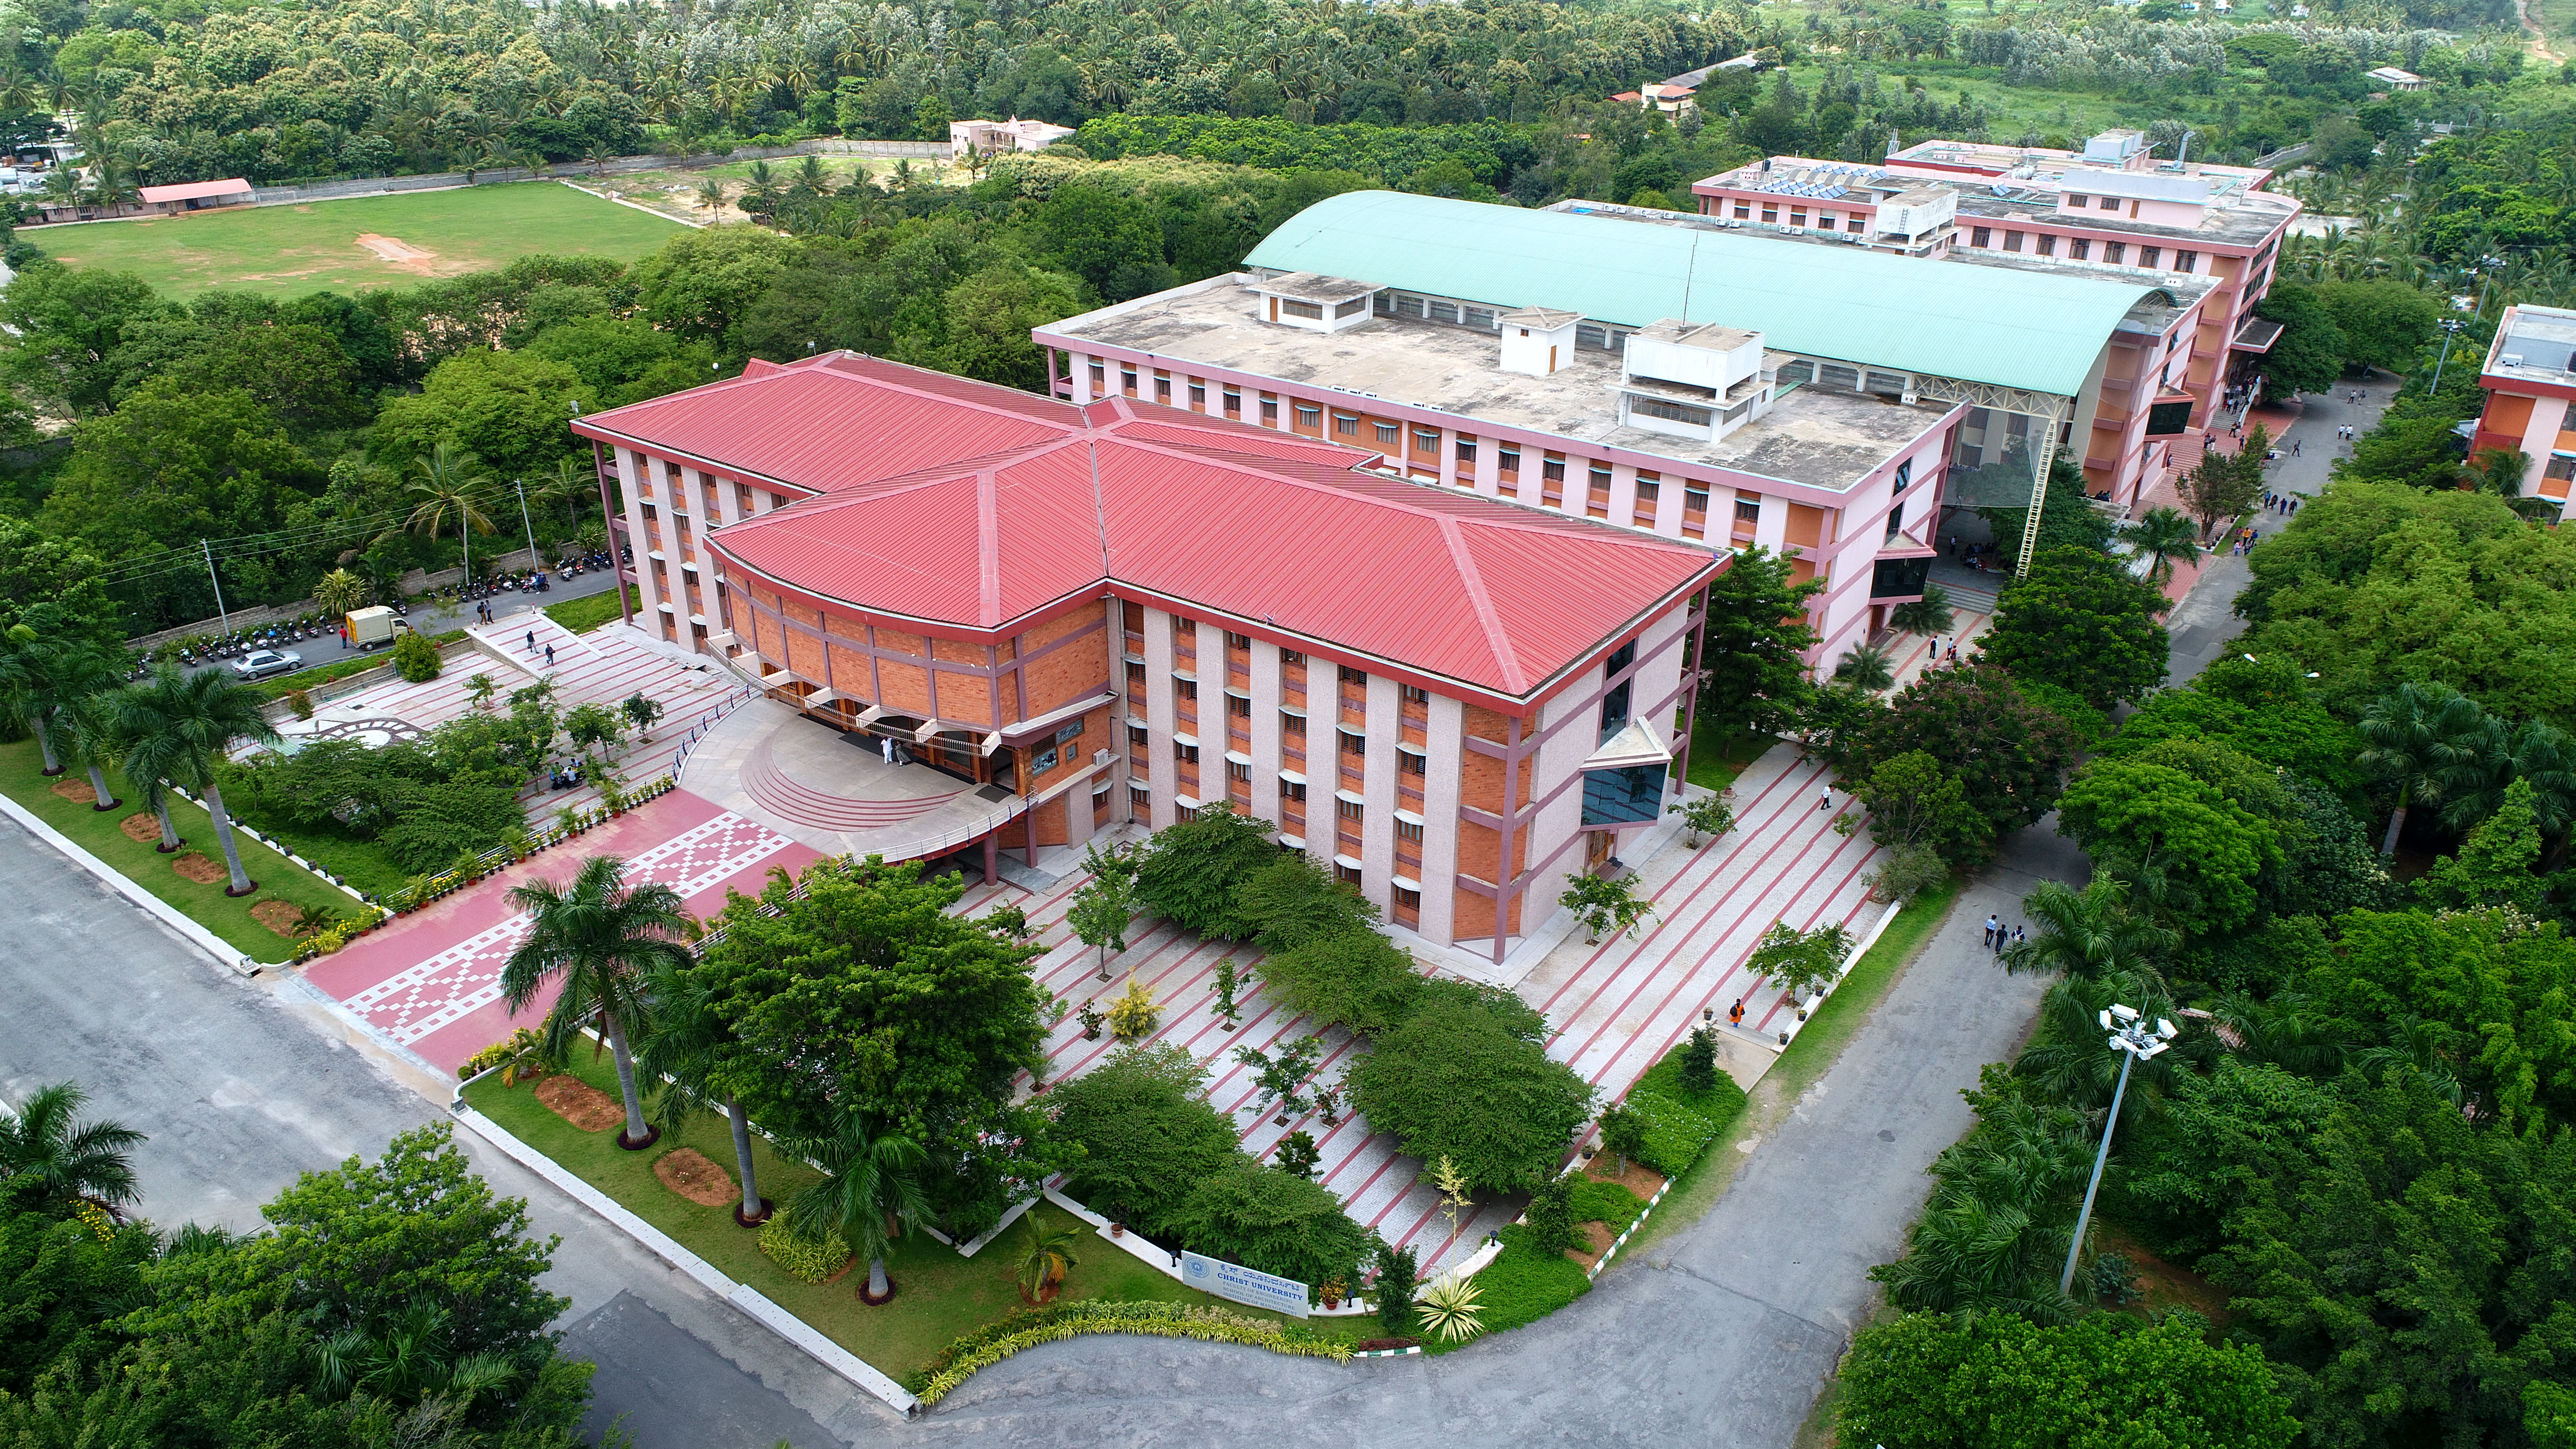
\includegraphics[width=\paperwidth,height=\paperheight]{assets/College.JPG}
        };
        \fill[white, opacity=0.9] (current page.south west) rectangle (current page.north east);
    \end{tikzpicture}
}
\begin{frame}
    \begin{center}
    \vspace*{1cm}

    \begin{tikzpicture}
        \node[draw=blue!20, line width=6pt, rounded corners=25pt, 
              fill=blue!10, inner sep=25pt, outer sep=25pt] {
            {\fontfamily{pzc}\fontsize{130}{250}\selectfont ~~~E-Portfolio~~~}
        };
    \end{tikzpicture}

    
    
    
    \vspace*{2cm}

 \begin{minipage}[t]{0.4\textwidth}
    \centering
    \begin{tikzpicture}
        \node[double=blue!30, double distance=4pt, draw=blue!80, line width=3pt,
              rounded corners=12pt, fill=blue!5, inner sep=2pt] {
            \includegraphics[width=0.5\textwidth]{\StudentPhoto}
        };
    \end{tikzpicture}
\end{minipage}

 
    \vspace*{3cm}

    \begin{tikzpicture}
        \node[draw=blue!20, line width=6pt, rounded corners=25pt, 
              fill=orange!10, inner sep=25pt, outer sep=25pt] {
            {\fontfamily{pzc}\fontsize{200}{250}\selectfont~~~\StudentName~~~}
        };
    \end{tikzpicture}

    \vspace*{2cm}

     \begin{tikzpicture}
        \node[draw=blue!20, line width=6pt, rounded corners=15pt, 
              fill=green!10, inner sep=25pt, outer sep=25pt] {
                \begin{minipage}{0.9\textwidth}
                  \centering
            \vspace*{2cm}
    {\fontsize{60}{250}\selectfont Register No: \StudentRegNo}\\
    \vspace*{2cm}
    {\fontsize{60}{250}\selectfont\StudentDepartment}\\
    \vspace*{1cm}
    {\fontsize{60}{250}\selectfont\CollegeName}\\
    \vspace*{1cm}
    {\fontsize{60}{250}\selectfont\UniversityName}\\
    \vspace*{1cm}
    {\fontsize{60}{250}\selectfont Academic Year: \AcademicYear}\\
    \end{minipage}
        };
    \end{tikzpicture}

    
  \end{center}


\end{frame}
}

 {\fontsize{40}{50}\selectfont

\begin{frame}[t]

\begin{columns}[t]
\separatorcolumn

\begin{column}{\colwidth}

\begin{exampleblock}{\LARGE{\textbf{SMART GOALS}}}

  \begin{enumerate}
  \varitem{red!40}{\textbf{1}} \justifying{\GoalOne}
  \varitem{cyan!40}{\textbf{2}} \justifying{\GoalTwo}
  \varitem{orange!40}{\textbf{3}} \justifying{\GoalThree}
  \end{enumerate}
\end{exampleblock}

\begin{block}{\LARGE{\textbf{ACADEMIC INFORMATIONS}}}
\vspace{-10px}
\begin{center}
  
\begin{tikzpicture}[scale=4]

\ifdefempty{\PGYear}{
  \draw[ultra thick, black!20] (0,-1) -- (0,4);
}{
\draw[ultra thick, black!20] (0,-1) -- (0,5);
\fill[blue!70] (0,4.5) circle (0.12);
\draw[blue!70, thick] (0,4.5) -- (1,4.5);
\node[blue!70, font=\bfseries] at (0,4.8) {\PGYear};
\fill[blue!20, rounded corners=8pt] (1.1,4.2) rectangle (2,4.8);
\node at (1.55,4.5) {\Huge\faTrophy};
\node[anchor=west, blue!70, font=\bfseries] at (2.2,4.65) {Master of Technology \PGStatus};
\node[anchor=west] at (2.2,4.35) {\PGSpecialization};
\node[anchor=west] at (2.2,4.0) {CGPA: \textbf{\PGCGPA}/\PGCGPAMax};
}

\fill[brown!70] (0,3.2) circle (0.12);
\draw[brown!70, thick] (0,3.2) -- (1,3.2);
\node[brown!70, font=\bfseries] at (0,3.5) {\UGYear};
\fill[brown!20, rounded corners=8pt] (1.1,2.9) rectangle (2,3.5);
\node at (1.55,3.2) {\Huge\faAward};
\node[anchor=west, brown!100, font=\bfseries] at (2.2,3.35) {Bachelor of Technology \UGStatus};
\node[anchor=west] at (2.2,3.05) {\UGSpecialization};
\node[anchor=west] at (2.2,2.7) {CGPA: \textbf{\UGCGPA}/\UGCGPAMax};

% 2022 Event - 3 lines with more spacing
\fill[purple!70] (0,1.7) circle (0.12);
\draw[purple!70, thick] (0,1.7) -- (1,1.7);
\node[purple!70, font=\bfseries] at (0,2.0) {\PUCYear};
\fill[purple!20, rounded corners=8pt] (1.1,1.4) rectangle (2,2.0);
\node at (1.55,1.7) {\Huge\faCertificate};
\node[anchor=west, purple!70, font=\bfseries] at (2.2,1.85) {PUC (\PUCSpecialization) \PUCStatus};
\node[anchor=west] at (2.2,1.55) {JSS Public School, Bangalore};
\node[anchor=west] at (2.2,1.2) {Passed with \textbf{\PUCMarks\%} score};

% 2021 Event - 3 lines with more spacing
\fill[cyan!70] (0,0.1) circle (0.12);
\draw[cyan!70, thick] (0,0.1) -- (1,0.1);
\node[cyan!70, font=\bfseries] at (0,0.4) {\MetriculationYear};
\fill[cyan!20, rounded corners=8pt] (1.1,-0.2) rectangle (2,0.4);
\node at (1.55,0.1) {\Huge\faStar};
\node[anchor=west, cyan!70, font=\bfseries] at (2.2,0.25) {Metriculation (\MetriculationBoard) \MetriculationStatus};
\node[anchor=west] at (2.2,-0.05) {\MetriculationSchool};
\node[anchor=west] at (2.2,-0.3) {Passed with \textbf{\MetriculationMarks\%} score};

\ifdefempty{\DiplomaYear}{
}{
% 2020 Event - 3 lines with more spacing
\fill[red!70] (0,-1.5) circle (0.12);
\draw[red!70, thick] (0,-1.5) -- (1,-1.5);
\node[red!70, font=\bfseries] at (0,-1.2) {\DiplomaYear};
\fill[red!20, rounded corners=8pt] (1.1,-1.8) rectangle (2,-1.2);
\node at (1.55,-1.5) {\Huge\faGraduationCap};
\node[anchor=west, red!70, font=\bfseries] at (2.2,-1.35) {Diploma(\DiplomaSpecilization) \DiplomaStatus};
\node[anchor=west] at (2.2,-1.65) {\DiplomaCollege};
\node[anchor=west] at (2.2,-1.9) {Passed with \textbf{\DiplomaMarks\%} score};
}
\end{tikzpicture}

\end{center}

  \end{block}


   \begin{exampleblock}{\LARGE{\textbf{DIGITAL IDENTITIES}}}
    \begin{center}

      \ifdefempty{\LinkedInURL}{}{
\href{\LinkedInURL}{\faLinkedin\ \textcolor{blue}{LinkedIn}} \quad}
\ifdefempty{\GithubURL}{}{
\href{\GithubURL}{\faGithub\ \textcolor{black}{GitHub}} \quad}
\ifdefempty{\TwitterURL}{}{
\href{\TwitterURL}{\faTwitter\ \textcolor{blue!60}{Twitter}} \quad}
\ifdefempty{\PortfolioURL}{}{
\href{\PortfolioURL}{\faGlobe\ \textcolor{green!60!black}{Portfolio}}} \quad
\ifdefempty{\OrcidURL}{}{
\href{\OrcidURL}{\faGlobe\ \textcolor{green!60!black}{Orcid}}} \quad
\ifdefempty{\GoogleScholarURL}{}{
\href{\GoogleScholarURL}{\faGlobe\ \textcolor{green!60!black}{Google Scholar}}} \quad
\end{center}


  \end{exampleblock}




  \begin{exampleblock}{}
    \vspace{-75px}
\begin{center}
  \href{\EmailID}{\faEnvelope\ \textcolor{black}{\EmailID}} \quad \\
\href{tel:\MobileNo}{\faMobile\ \textcolor{black}{\MobileNo}}
  

\end{center}
    
\end{exampleblock}



  \begin{block}{\LARGE{\textbf{AREAS OF INTEREST}}}
    \begin{center}
      \ifdefempty{\AreaOfInterestOne}{}{
        \begin{tikzpicture}
        \node[draw=blue!20, line width=6pt, rounded corners=25pt, 
              fill=blue!10, inner sep=25pt, outer sep=25pt] {
            {\fontfamily{pzc}\fontsize{50}{100}\selectfont ~~~\AreaOfInterestOne~~~}
        };
    \end{tikzpicture} \quad}
      \ifdefempty{\AreaOfInterestTwo}{}{
        \begin{tikzpicture}
        \node[draw=red!20, line width=6pt, rounded corners=25pt, 
              fill=orange!10, inner sep=25pt, outer sep=25pt] {
            {\fontfamily{pzc}\fontsize{50}{100}\selectfont ~~~\AreaOfInterestTwo~~~}
        };
    \end{tikzpicture}   \quad} 
      \ifdefempty{\AreaOfInterestThree}{}{
        \begin{tikzpicture}
        \node[draw=blue!20, line width=6pt, rounded corners=25pt, 
              fill=green!10, inner sep=25pt, outer sep=25pt] {
            {\fontfamily{pzc}\fontsize{50}{100}\selectfont ~~~\AreaOfInterestThree~~~}
        };
    \end{tikzpicture} \quad}

    \end{center}
  \end{block}

\end{column}

\separatorcolumn

\begin{column}{\colwidth}

  \begin{block}{\LARGE{\textbf{TECHNOLOGIES/TOOLS}}}

   \vspace{0.6cm} 
    
\begin{minipage}{0.95\textwidth}
\LARGE

\ifdefempty{\TechnologyToolOne}{}{
\colorbox{red!30}{\makebox[10cm]{\textcolor{red}{\rule{\TechnologyToolOneValue cm}{1cm}}}}\hfill
\TechnologyToolOne \hfill
\vspace{0.4cm}
}

\ifdefempty{\TechnologyToolTwo}{}{
\colorbox{purple!30}{\makebox[10cm]{\textcolor{purple}{\rule{\TechnologyToolTwoValue cm}{1cm}}}}\hfill
\TechnologyToolTwo\hfill
\vspace{0.4cm}
}

\ifdefempty{\TechnologyToolThree}{}{
\colorbox{orange!30}{\makebox[10cm]{\textcolor{orange}{\rule{\TechnologyToolThreeValue cm}{1cm}}}}\hfill
\TechnologyToolThree\hfill
\vspace{0.4cm}
}


\ifdefempty{\TechnologyToolFour}{}{
\colorbox{teal!30}{\makebox[10cm]{\textcolor{teal}{\rule{\TechnologyToolFourValue cm}{1cm}}}}\hfill
\TechnologyToolFour\hfill
\vspace{0.4cm}
}

\ifdefempty{\TechnologyToolFive}{}{
\colorbox{cyan!30}{\makebox[10cm]{\textcolor{cyan}{\rule{\TechnologyToolFiveValue cm}{1cm}}}}\hfill
\TechnologyToolFive\hfill
\vspace{0.4cm}
}

\ifdefempty{\TechnologyToolSix}{}{
\colorbox{gray!30}{\makebox[10cm]{\textcolor{gray}{\rule{\TechnologyToolSixValue cm}{1cm}}}}\hfill
\TechnologyToolSix\hfill
\vspace{0.4cm}
}

\ifdefempty{\TechnologyToolSeven}{}{
\colorbox{orange!30}{\makebox[10cm]{\textcolor{gray}{\rule{\TechnologyToolSevenValue cm}{1cm}}}}\hfill
\TechnologyToolSeven\hfill
\vspace{0.4cm}
}


\ifdefempty{\TechnologyToolEight}{}{
\colorbox{red!30}{\makebox[10cm]{\textcolor{gray}{\rule{\TechnologyToolEightValue cm}{1cm}}}}\hfill
\TechnologyToolEight\hfill
\vspace{0.4cm}
}

\end{minipage}

\vspace{2cm}
  \end{block}

  \begin{exampleblock}{\LARGE{\textbf{SKILLS}}}


\begin{center}

\vspace{1cm}

\begin{tikzpicture}[scale=1.8]
    % Define colors
    \definecolor{set1}{RGB}{255,100,100}
    \definecolor{set2}{RGB}{100,255,100}
    \definecolor{set3}{RGB}{100,100,255}
    \definecolor{set4}{RGB}{255,255,100}
    
    % Draw four overlapping circles in radial arrangement
    \fill[set1, opacity=0.7] (45:2) circle (\SkillOneValue);
    \fill[set2, opacity=0.7] (135:2) circle (\SkillTwoValue);
    \fill[set3, opacity=0.7] (225:2) circle (\SkillThreeValue);
    \fill[set4, opacity=0.7] (315:2) circle (\SkillFourValue);
    
    % Set labels
    \node at (45:4.5) {\Large \SkillOne};
    \node at (135:4.5) {\Large \SkillTwo};
    \node at (225:4.5) {\Large \SkillThree};
    \node at (315:4.5) {\Large \SkillFour};
    
\end{tikzpicture}
\end{center}
\vspace{2cm}

   
  \end{exampleblock}


     \vspace{0.6cm} 

  \begin{block}{\LARGE{\textbf{ACHIEVEMENTS AND RESPONSIBILITIES}}}

\begin{table}
\centering
\rowcolors{2}{blue!5}{white}
\begin{tabular}{p{23cm} p{30cm}}
\toprule
\rowcolor{blue!60}
\textcolor{white}{\textbf{Achievment/Role}}  & 
\textcolor{white}{\textbf{Responsibilities}}  \\
\midrule
\AchievmentRoleResponsibility
\bottomrule
\end{tabular}
\end{table}

  \end{block}

\end{column}

\separatorcolumn
\end{columns}
\end{frame}



\ifdefempty{\ProjectTitleOne}{}{
\begin{frame}[t]

\begin{columns}[t]

\separatorcolumn

\begin{column}{\colwidth}

  \begin{block}{\LARGE{\textbf{PROJECTS}}}

   \begin{enumerate}
  \varitem{cyan!40}{\textbf{1}} 
  
  \justifying{\textbf{Project Title:} \ProjectTitleOne}\\
  \vspace{1cm}
  \textbf{Description:} \ProjectDescriptionOne\\
  \vspace{1cm}
  \begin{figure}
      \centering
      \begin{center}
        \includegraphics[scale=\ProjectImageFirstScaleOne]{\ProjectImageFirstOne}
        \caption{\ProjectImageFirstCaptionOne}
        \label{fig3}
      \end{center}
    \end{figure}

    \begin{figure}
      \centering
      \begin{center}
        \includegraphics[scale=\ProjectImageSecondScaleOne]{\ProjectImageSecondOne}
        \caption{\ProjectImageSecondCaptionOne}
        \label{fig4}
      \end{center}
    \end{figure}
    \textbf{Outcome:} \ProjectOutcomeOne
\end{enumerate}
  

  \end{block}

\end{column}

 \separatorcolumn

\ifdefempty{\ProjectTitleTwo}{}{
  \begin{column}{\colwidth}

  \begin{block}{\LARGE{\textbf{PROJECTS}}}

   \begin{enumerate}
  \varitem{cyan!40}{\textbf{2}} 
  
  \justifying{\textbf{Project Title:} \ProjectTitleTwo}\\
  \vspace{1cm}
  \textbf{Description:} \ProjectDescriptionTwo\\
  \vspace{1cm}
  \begin{figure}
      \centering
      \begin{center}
        \includegraphics[scale=\ProjectImageFirstScaleTwo]{\ProjectImageFirstTwo}
        \caption{\ProjectImageFirstCaptionTwo}
        \label{fig3}
      \end{center}
    \end{figure}

    \begin{figure}
      \centering
      \begin{center}
        \includegraphics[scale=\ProjectImageSecondScaleTwo]{\ProjectImageSecondTwo}
        \caption{\ProjectImageSecondCaptionTwo}
        \label{fig4}
      \end{center}
    \end{figure}
    \textbf{Outcome:} \ProjectOutcomeTwo
\end{enumerate}
  

  \end{block}

\end{column}
}

\separatorcolumn
\end{columns}
\end{frame}
}

\ifdefempty{\ProjectTitleThree}{}{
\begin{frame}[t]

\begin{columns}[t]

\separatorcolumn

\begin{column}{\colwidth}

  \begin{block}{\LARGE{\textbf{PROJECTS}}}

   \begin{enumerate}
  \varitem{cyan!40}{\textbf{3}} 
  
  \justifying{\textbf{Project Title:} \ProjectTitleThree}\\
  \vspace{1cm}
  \textbf{Description:} \ProjectDescriptionThree\\
  \vspace{1cm}
  \begin{figure}
      \centering
      \begin{center}
        \includegraphics[scale=\ProjectImageFirstScaleThree]{\ProjectImageFirstThree}
        \caption{\ProjectImageFirstCaptionThree}
        \label{fig5}
      \end{center}
    \end{figure}

    \begin{figure}
      \centering
      \begin{center}
        \includegraphics[scale=\ProjectImageSecondScaleThree]{\ProjectImageSecondThree}
        \caption{\ProjectImageSecondCaptionThree}
        \label{fig6}
      \end{center}
    \end{figure}
    \textbf{Outcome:} \ProjectOutcomeThree
\end{enumerate}
  

  \end{block}

\end{column}

\separatorcolumn

\ifdefempty{\ProjectTitleFour}{}{
  \begin{column}{\colwidth}

  \begin{block}{\LARGE{\textbf{PROJECTS}}}

   \begin{enumerate}
  \varitem{cyan!40}{\textbf{4}} 
  
  \justifying{\textbf{Project Title:} \ProjectTitleFour}\\
  \vspace{1cm}
  \textbf{Description:} \ProjectDescriptionFour\\
  \vspace{1cm}
  \begin{figure}
      \centering
      \begin{center}
        \includegraphics[scale=\ProjectImageFirstScaleFour]{\ProjectImageFirstFour}
        \caption{\ProjectImageFirstCaptionFour}
        \label{fig7}
      \end{center}
    \end{figure}

    \begin{figure}
      \centering
      \begin{center}
        \includegraphics[scale=\ProjectImageSecondScaleFour]{\ProjectImageSecondFour}
        \caption{\ProjectImageSecondCaptionFour}
        \label{fig8}
      \end{center}
    \end{figure}
    \textbf{Outcome:} \ProjectOutcomeFour
\end{enumerate}
  

  \end{block}

\end{column}
}

\separatorcolumn
\end{columns}
\end{frame}
}


\ifdefempty{\ProjectTitleFive}{}{
\begin{frame}[t]

\begin{columns}[t]

\separatorcolumn

\begin{column}{\colwidth}

  \begin{block}{\LARGE{\textbf{PROJECTS}}}

   \begin{enumerate}
  \varitem{cyan!40}{\textbf{5}} 
  
  \justifying{\textbf{Project Title:} \ProjectTitleFive}\\
  \vspace{1cm}
  \textbf{Description:} \ProjectDescriptionFive\\
  \vspace{1cm}
  \begin{figure}
      \centering
      \begin{center}
        \includegraphics[scale=\ProjectImageFirstScaleFive]{\ProjectImageFirstFive}
        \caption{\ProjectImageFirstCaptionFive}
        \label{fig9}
      \end{center}
    \end{figure}

    \begin{figure}
      \centering
      \begin{center}
        \includegraphics[scale=\ProjectImageSecondScaleFive]{\ProjectImageSecondFive}
        \caption{\ProjectImageSecondCaptionFive}
        \label{fig10}
      \end{center}
    \end{figure}
    \textbf{Outcome:} \ProjectOutcomeFive
\end{enumerate}
  

  \end{block}

\end{column}

\separatorcolumn

\ifdefempty{\ProjectTitleSix}{}{
  \begin{column}{\colwidth}

  \begin{block}{\LARGE{\textbf{PROJECTS}}}

   \begin{enumerate}
  \varitem{cyan!40}{\textbf{6}} 
  
  \justifying{\textbf{Project Title:} \ProjectTitleSix}\\
  \vspace{1cm}
  \textbf{Description:} \ProjectDescriptionSix\\
  \vspace{1cm}
  \begin{figure}
      \centering
      \begin{center}
        \includegraphics[scale=\ProjectImageFirstScaleSix]{\ProjectImageFirstSix}
        \caption{\ProjectImageFirstCaptionSix}
        \label{fig11}
      \end{center}
    \end{figure}

    \begin{figure}
      \centering
      \begin{center}
        \includegraphics[scale=\ProjectImageSecondScaleSix]{\ProjectImageSecondSix}
        \caption{\ProjectImageSecondCaptionSix}
        \label{fig12}
      \end{center}
    \end{figure}
    \textbf{Outcome:} \ProjectOutcomeSix
\end{enumerate}
  

  \end{block}

\end{column}
}

\separatorcolumn
\end{columns}
\end{frame}
}

\ifdefempty{\ProjectTitleSeven}{}{
\begin{frame}[t]

\begin{columns}[t]

\separatorcolumn

\begin{column}{\colwidth}

  \begin{block}{\LARGE{\textbf{PROJECTS}}}

   \begin{enumerate}
  \varitem{cyan!40}{\textbf{7}} 
  
  \justifying{\textbf{Project Title:} \ProjectTitleSeven}\\
  \vspace{1cm}
  \textbf{Description:} \ProjectDescriptionSeven\\
  \vspace{1cm}
  \begin{figure}
      \centering
      \begin{center}
        \includegraphics[scale=\ProjectImageFirstScaleSeven]{\ProjectImageFirstSeven}
        \caption{\ProjectImageFirstCaptionSeven}
        \label{fig13}
      \end{center}
    \end{figure}

    \begin{figure}
      \centering
      \begin{center}
        \includegraphics[scale=\ProjectImageSecondScaleSeven]{\ProjectImageSecondSeven}
        \caption{\ProjectImageSecondCaptionSeven}
        \label{fig14}
      \end{center}
    \end{figure}
    \textbf{Outcome:} \ProjectOutcomeSeven
\end{enumerate}
  

  \end{block}

\end{column}

\separatorcolumn

\ifdefempty{\ProjectTitleEight}{}{
  \begin{column}{\colwidth}

  \begin{block}{\LARGE{\textbf{PROJECTS}}}

   \begin{enumerate}
  \varitem{cyan!40}{\textbf{8}} 
  
  \justifying{\textbf{Project Title:} \ProjectTitleEight}\\
  \vspace{1cm}
  \textbf{Description:} \ProjectDescriptionEight\\
  \vspace{1cm}
  \begin{figure}
      \centering
      \begin{center}
        \includegraphics[scale=\ProjectImageFirstScaleEight]{\ProjectImageFirstEight}
        \caption{\ProjectImageFirstCaptionEight}
        \label{fig15}
      \end{center}
    \end{figure}

    \begin{figure}
      \centering
      \begin{center}
        \includegraphics[scale=\ProjectImageSecondScaleEight]{\ProjectImageSecondEight}
        \caption{\ProjectImageSecondCaptionEight}
        \label{fig16}
      \end{center}
    \end{figure}
    \textbf{Outcome:} \ProjectOutcomeEight
\end{enumerate}
  

  \end{block}

\end{column}
}

\separatorcolumn
\end{columns}
\end{frame}
}

\ifdefempty{\ProjectTitleNine}{}{
\begin{frame}[t]

\begin{columns}[t]

\separatorcolumn

\begin{column}{\colwidth}

  \begin{block}{\LARGE{\textbf{PROJECTS}}}

   \begin{enumerate}
  \varitem{cyan!40}{\textbf{9}} 
  
  \justifying{\textbf{Project Title:} \ProjectTitleNine}\\
  \vspace{1cm}
  \textbf{Description:} \ProjectDescriptionNine\\
  \vspace{1cm}
  \begin{figure}
      \centering
      \begin{center}
        \includegraphics[scale=\ProjectImageFirstScaleNine]{\ProjectImageFirstNine}
        \caption{\ProjectImageFirstCaptionNine}
        \label{fig17}
      \end{center}
    \end{figure}

    \begin{figure}
      \centering
      \begin{center}
        \includegraphics[scale=\ProjectImageSecondScaleNine]{\ProjectImageSecondNine}
        \caption{\ProjectImageSecondCaptionNine}
        \label{fig18}
      \end{center}
    \end{figure}
    \textbf{Outcome:} \ProjectOutcomeNine
\end{enumerate}
  

  \end{block}

\end{column}

\separatorcolumn

\ifdefempty{\ProjectTitleTen}{}{
  \begin{column}{\colwidth}

  \begin{block}{\LARGE{\textbf{PROJECTS}}}

   \begin{enumerate}
  \varitem{cyan!40}{\textbf{10}} 
  
  \justifying{\textbf{Project Title:} \ProjectTitleTen}\\
  \vspace{1cm}
  \textbf{Description:} \ProjectDescriptionTen\\
  \vspace{1cm}
  \begin{figure}
      \centering
      \begin{center}
        \includegraphics[scale=\ProjectImageFirstScaleTen]{\ProjectImageFirstTen}
        \caption{\ProjectImageFirstCaptionTen}
        \label{fig19}
      \end{center}
    \end{figure}

    \begin{figure}
      \centering
      \begin{center}
        \includegraphics[scale=\ProjectImageSecondScaleTen]{\ProjectImageSecondTen}
        \caption{\ProjectImageSecondCaptionTen}
        \label{fig20}
      \end{center}
    \end{figure}
    \textbf{Outcome:} \ProjectOutcomeTen
\end{enumerate}
  

  \end{block}

\end{column}
}

\separatorcolumn
\end{columns}
\end{frame}
}

\ifdefempty{\ResearchTitleOne}{}{
\begin{frame}[t]

\begin{columns}[t]

\separatorcolumn

\begin{column}{\colwidth}

  \begin{block}{\LARGE{\textbf{RESEARCH WORK}}}

   \begin{enumerate}
  \varitem{cyan!40}{\textbf{1}} 
  
  \justifying{\textbf{Research Title:} \ResearchTitleOne}\\
  \vspace{1cm}
  \textbf{Description:} \ResearchDescriptionOne\\
  \vspace{1cm}
  \begin{figure}
      \centering
      \begin{center}
        \includegraphics[scale=\ResearchImageFirstScaleOne]{\ResearchImageFirstOne}
        \caption{\ResearchImageFirstCaptionOne}
        \label{fig:research1-1}
      \end{center}
    \end{figure}

    \begin{figure}
      \centering
      \begin{center}
        \includegraphics[scale=\ResearchImageSecondScaleOne]{\ResearchImageSecondOne}
        \caption{\ResearchImageSecondCaptionOne}
        \label{fig:research1-2}
      \end{center}
    \end{figure}
    \textbf{Findings:} \ResearchOutcomeOne
\end{enumerate}
  

  \end{block}

\end{column}

 \separatorcolumn

\ifdefempty{\ResearchTitleTwo}{}{
  \begin{column}{\colwidth}

  \begin{block}{\LARGE{\textbf{RESEARCH WORK}}}

   \begin{enumerate}
  \varitem{cyan!40}{\textbf{2}} 
  
  \justifying{\textbf{Research Title:} \ResearchTitleTwo}\\
  \vspace{1cm}
  \textbf{Description:} \ResearchDescriptionTwo\\
  \vspace{1cm}
  \begin{figure}
      \centering
      \begin{center}
        \includegraphics[scale=\ResearchImageFirstScaleTwo]{\ResearchImageFirstTwo}
        \caption{\ResearchImageFirstCaptionTwo}
        \label{fig:research2-1}
      \end{center}
    \end{figure}

    \begin{figure}
      \centering
      \begin{center}
        \includegraphics[scale=\ResearchImageSecondScaleTwo]{\ResearchImageSecondTwo}
        \caption{\ResearchImageSecondCaptionTwo}
        \label{fig:research2-2}
      \end{center}
    \end{figure}
    \textbf{Findings:} \ResearchOutcomeTwo
\end{enumerate}
  

  \end{block}

\end{column}
}

\separatorcolumn
\end{columns}
\end{frame}
}

\ifdefempty{\ResearchTitleThree}{}{
\begin{frame}[t]

\begin{columns}[t]

\separatorcolumn

\begin{column}{\colwidth}

  \begin{block}{\LARGE{\textbf{RESEARCH WORK}}}

   \begin{enumerate}
  \varitem{cyan!40}{\textbf{3}} 
  
  \justifying{\textbf{Research Title:} \ResearchTitleThree}\\
  \vspace{1cm}
  \textbf{Description:} \ResearchDescriptionThree\\
  \vspace{1cm}
  \begin{figure}
      \centering
      \begin{center}
        \includegraphics[scale=\ResearchImageFirstScaleThree]{\ResearchImageFirstThree}
        \caption{\ResearchImageFirstCaptionThree}
        \label{fig:research3-1}
      \end{center}
    \end{figure}

    \begin{figure}
      \centering
      \begin{center}
        \includegraphics[scale=\ResearchImageSecondScaleThree]{\ResearchImageSecondThree}
        \caption{\ResearchImageSecondCaptionThree}
        \label{fig:research3-2}
      \end{center}
    \end{figure}
    \textbf{Findings:} \ResearchOutcomeThree
\end{enumerate}
  

  \end{block}

\end{column}

 \separatorcolumn

\ifdefempty{\ResearchTitleFour}{}{
  \begin{column}{\colwidth}

  \begin{block}{\LARGE{\textbf{RESEARCH WORK}}}

   \begin{enumerate}
  \varitem{cyan!40}{\textbf{4}} 
  
  \justifying{\textbf{Research Title:} \ResearchTitleFour}\\
  \vspace{1cm}
  \textbf{Description:} \ResearchDescriptionFour\\
  \vspace{1cm}
  \begin{figure}
      \centering
      \begin{center}
        \includegraphics[scale=\ResearchImageFirstScaleFour]{\ResearchImageFirstFour}
        \caption{\ResearchImageFirstCaptionFour}
        \label{fig:research4-1}
      \end{center}
    \end{figure}

    \begin{figure}
      \centering
      \begin{center}
        \includegraphics[scale=\ResearchImageSecondScaleFour]{\ResearchImageSecondFour}
        \caption{\ResearchImageSecondCaptionFour}
        \label{fig:research4-2}
      \end{center}
    \end{figure}
    \textbf{Findings:} \ResearchOutcomeFour
\end{enumerate}
  

  \end{block}

\end{column}
}

\separatorcolumn
\end{columns}
\end{frame}
}

\ifdefempty{\ResearchTitleFive}{}{
\begin{frame}[t]

\begin{columns}[t]

\separatorcolumn

\begin{column}{\colwidth}

  \begin{block}{\LARGE{\textbf{RESEARCH WORK}}}

   \begin{enumerate}
  \varitem{cyan!40}{\textbf{5}} 
  
  \justifying{\textbf{Research Title:} \ResearchTitleFive}\\
  \vspace{1cm}
  \textbf{Description:} \ResearchDescriptionFive\\
  \vspace{1cm}
  \begin{figure}
      \centering
      \begin{center}
        \includegraphics[scale=\ResearchImageFirstScaleFive]{\ResearchImageFirstFive}
        \caption{\ResearchImageFirstCaptionFive}
        \label{fig:research5-1}
      \end{center}
    \end{figure}

    \begin{figure}
      \centering
      \begin{center}
        \includegraphics[scale=\ResearchImageSecondScaleFive]{\ResearchImageSecondFive}
        \caption{\ResearchImageSecondCaptionFive}
        \label{fig:research5-2}
      \end{center}
    \end{figure}
    \textbf{Findings:} \ResearchOutcomeFive
\end{enumerate}
  

  \end{block}

\end{column}

 \separatorcolumn

\ifdefempty{\ResearchTitleSix}{}{
  \begin{column}{\colwidth}

  \begin{block}{\LARGE{\textbf{RESEARCH WORK}}}

   \begin{enumerate}
  \varitem{cyan!40}{\textbf{6}} 
  
  \justifying{\textbf{Research Title:} \ResearchTitleSix}\\
  \vspace{1cm}
  \textbf{Description:} \ResearchDescriptionSix\\
  \vspace{1cm}
  \begin{figure}
      \centering
      \begin{center}
        \includegraphics[scale=\ResearchImageFirstScaleSix]{\ResearchImageFirstSix}
        \caption{\ResearchImageFirstCaptionSix}
        \label{fig:research6-1}
      \end{center}
    \end{figure}

    \begin{figure}
      \centering
      \begin{center}
        \includegraphics[scale=\ResearchImageSecondScaleSix]{\ResearchImageSecondSix}
        \caption{\ResearchImageSecondCaptionSix}
        \label{fig:research6-2}
      \end{center}
    \end{figure}
    \textbf{Findings:} \ResearchOutcomeSix
\end{enumerate}
  

  \end{block}

\end{column}
}

\separatorcolumn
\end{columns}
\end{frame}
}

\ifdefempty{\ResearchTitleSeven}{}{
\begin{frame}[t]

\begin{columns}[t]

\separatorcolumn

\begin{column}{\colwidth}

  \begin{block}{\LARGE{\textbf{RESEARCH WORK}}}

   \begin{enumerate}
  \varitem{cyan!40}{\textbf{7}} 
  
  \justifying{\textbf{Research Title:} \ResearchTitleSeven}\\
  \vspace{1cm}
  \textbf{Description:} \ResearchDescriptionSeven\\
  \vspace{1cm}
  \begin{figure}
      \centering
      \begin{center}
        \includegraphics[scale=\ResearchImageFirstScaleSeven]{\ResearchImageFirstSeven}
        \caption{\ResearchImageFirstCaptionSeven}
        \label{fig:research7-1}
      \end{center}
    \end{figure}

    \begin{figure}
      \centering
      \begin{center}
        \includegraphics[scale=\ResearchImageSecondScaleSeven]{\ResearchImageSecondSeven}
        \caption{\ResearchImageSecondCaptionSeven}
        \label{fig:research7-2}
      \end{center}
    \end{figure}
    \textbf{Findings:} \ResearchOutcomeSeven
\end{enumerate}
  

  \end{block}

\end{column}

 \separatorcolumn

\ifdefempty{\ResearchTitleEight}{}{
  \begin{column}{\colwidth}

  \begin{block}{\LARGE{\textbf{RESEARCH WORK}}}

   \begin{enumerate}
  \varitem{cyan!40}{\textbf{8}} 
  
  \justifying{\textbf{Research Title:} \ResearchTitleEight}\\
  \vspace{1cm}
  \textbf{Description:} \ResearchDescriptionEight\\
  \vspace{1cm}
  \begin{figure}
      \centering
      \begin{center}
        \includegraphics[scale=\ResearchImageFirstScaleEight]{\ResearchImageFirstEight}
        \caption{\ResearchImageFirstCaptionEight}
        \label{fig:research8-1}
      \end{center}
    \end{figure}

    \begin{figure}
      \centering
      \begin{center}
        \includegraphics[scale=\ResearchImageSecondScaleEight]{\ResearchImageSecondEight}
        \caption{\ResearchImageSecondCaptionEight}
        \label{fig:research8-2}
      \end{center}
    \end{figure}
    \textbf{Findings:} \ResearchOutcomeEight
\end{enumerate}
  

  \end{block}

\end{column}
}

\separatorcolumn
\end{columns}
\end{frame}
}

\ifdefempty{\ResearchTitleNine}{}{
\begin{frame}[t]

\begin{columns}[t]

\separatorcolumn

\begin{column}{\colwidth}

  \begin{block}{\LARGE{\textbf{RESEARCH WORK}}}

   \begin{enumerate}
  \varitem{cyan!40}{\textbf{9}} 
  
  \justifying{\textbf{Research Title:} \ResearchTitleNine}\\
  \vspace{1cm}
  \textbf{Description:} \ResearchDescriptionNine\\
  \vspace{1cm}
  \begin{figure}
      \centering
      \begin{center}
        \includegraphics[scale=\ResearchImageFirstScaleNine]{\ResearchImageFirstNine}
        \caption{\ResearchImageFirstCaptionNine}
        \label{fig:research9-1}
      \end{center}
    \end{figure}

    \begin{figure}
      \centering
      \begin{center}
        \includegraphics[scale=\ResearchImageSecondScaleNine]{\ResearchImageSecondNine}
        \caption{\ResearchImageSecondCaptionNine}
        \label{fig:research9-2}
      \end{center}
    \end{figure}
    \textbf{Findings:} \ResearchOutcomeNine
\end{enumerate}
  

  \end{block}

\end{column}

 \separatorcolumn

\ifdefempty{\ResearchTitleTen}{}{
  \begin{column}{\colwidth}

  \begin{block}{\LARGE{\textbf{RESEARCH WORK}}}

   \begin{enumerate}
  \varitem{cyan!40}{\textbf{10}} 
  
  \justifying{\textbf{Research Title:} \ResearchTitleTen}\\
  \vspace{1cm}
  \textbf{Description:} \ResearchDescriptionTen\\
  \vspace{1cm}
  \begin{figure}
      \centering
      \begin{center}
        \includegraphics[scale=\ResearchImageFirstScaleTen]{\ResearchImageFirstTen}
        \caption{\ResearchImageFirstCaptionTen}
        \label{fig:research10-1}
      \end{center}
    \end{figure}

    \begin{figure}
      \centering
      \begin{center}
        \includegraphics[scale=\ResearchImageSecondScaleTen]{\ResearchImageSecondTen}
        \caption{\ResearchImageSecondCaptionTen}
        \label{fig:research10-2}
      \end{center}
    \end{figure}
    \textbf{Findings:} \ResearchOutcomeTen
\end{enumerate}
  

  \end{block}

\end{column}
}

\separatorcolumn
\end{columns}
\end{frame}
}

\ifdefempty{\ActivityTitleOne}{}{
\begin{frame}[t]

\begin{columns}[t]

\separatorcolumn

\begin{column}{\colwidth}

  \begin{block}{\LARGE{\textbf{ACTIVITIES}}}

   \begin{enumerate}
  \varitem{cyan!40}{\textbf{1}} 
  
  \justifying{\textbf{Activity Title:} \ActivityTitleOne}\\
  \vspace{1cm}
  \textbf{Description:} \ActivityDescriptionOne\\
  \vspace{1cm}
  \begin{figure}
      \centering
      \begin{center}
        \includegraphics[scale=\ActivityImageFirstScaleOne]{\ActivityImageFirstOne}
        \caption{\ActivityImageFirstCaptionOne}
        \label{fig:activity1-1}
      \end{center}
    \end{figure}

    \begin{figure}
      \centering
      \begin{center}
        \includegraphics[scale=\ActivityImageSecondScaleOne]{\ActivityImageSecondOne}
        \caption{\ActivityImageSecondCaptionOne}
        \label{fig:activity1-2}
      \end{center}
    \end{figure}
    \textbf{Outcome:} \ActivityOutcomeOne
\end{enumerate}
  

  \end{block}

\end{column}

 \separatorcolumn

\ifdefempty{\ActivityTitleTwo}{}{
  \begin{column}{\colwidth}

  \begin{block}{\LARGE{\textbf{ACTIVITIES}}}

   \begin{enumerate}
  \varitem{cyan!40}{\textbf{2}} 
  
  \justifying{\textbf{Activity Title:} \ActivityTitleTwo}\\
  \vspace{1cm}
  \textbf{Description:} \ActivityDescriptionTwo\\
  \vspace{1cm}
  \begin{figure}
      \centering
      \begin{center}
        \includegraphics[scale=\ActivityImageFirstScaleTwo]{\ActivityImageFirstTwo}
        \caption{\ActivityImageFirstCaptionTwo}
        \label{fig:activity2-1}
      \end{center}
    \end{figure}

    \begin{figure}
      \centering
      \begin{center}
        \includegraphics[scale=\ActivityImageSecondScaleTwo]{\ActivityImageSecondTwo}
        \caption{\ActivityImageSecondCaptionTwo}
        \label{fig:activity2-2}
      \end{center}
    \end{figure}
    \textbf{Outcome:} \ActivityOutcomeTwo
\end{enumerate}
  

  \end{block}

\end{column}
}

\separatorcolumn
\end{columns}
\end{frame}
}


\ifdefempty{\ActivityTitleThree}{}{
\begin{frame}[t]

\begin{columns}[t]

\separatorcolumn

\begin{column}{\colwidth}

  \begin{block}{\LARGE{\textbf{ACTIVITIES}}}

   \begin{enumerate}
  \varitem{cyan!40}{\textbf{3}} 
  
  \justifying{\textbf{Activity Title:} \ActivityTitleThree}\\
  \vspace{1cm}
  \textbf{Description:} \ActivityDescriptionThree\\
  \vspace{1cm}
  \begin{figure}
      \centering
      \begin{center}
        \includegraphics[scale=\ActivityImageFirstScaleThree]{\ActivityImageFirstThree}
        \caption{\ActivityImageFirstCaptionThree}
        \label{fig:activity3-1}
      \end{center}
    \end{figure}

    \begin{figure}
      \centering
      \begin{center}
        \includegraphics[scale=\ActivityImageSecondScaleThree]{\ActivityImageSecondThree}
        \caption{\ActivityImageSecondCaptionThree}
        \label{fig:activity3-2}
      \end{center}
    \end{figure}
    \textbf{Outcome:} \ActivityOutcomeThree
\end{enumerate}
  

  \end{block}

\end{column}

 \separatorcolumn

\ifdefempty{\ActivityTitleFour}{}{
  \begin{column}{\colwidth}

  \begin{block}{\LARGE{\textbf{ACTIVITIES}}}

   \begin{enumerate}
  \varitem{cyan!40}{\textbf{4}} 
  
  \justifying{\textbf{Activity Title:} \ActivityTitleFour}\\
  \vspace{1cm}
  \textbf{Description:} \ActivityDescriptionFour\\
  \vspace{1cm}
  \begin{figure}
      \centering
      \begin{center>
        \includegraphics[scale=\ActivityImageFirstScaleFour]{\ActivityImageFirstFour}
        \caption{\ActivityImageFirstCaptionFour}
        \label{fig:activity4-1}
      \end{center}
    \end{figure}

    \begin{figure}
      \centering
      \begin{center}
        \includegraphics[scale=\ActivityImageSecondScaleFour]{\ActivityImageSecondFour}
        \caption{\ActivityImageSecondCaptionFour}
        \label{fig:activity4-2}
      \end{center}
    \end{figure}
    \textbf{Outcome:} \ActivityOutcomeFour
\end{enumerate}
  

  \end{block}

\end{column}
}

\separatorcolumn
\end{columns}
\end{frame}
}


\ifdefempty{\ActivityTitleFive}{}{
\begin{frame}[t]

\begin{columns}[t]

\separatorcolumn

\begin{column}{\colwidth}

  \begin{block}{\LARGE{\textbf{ACTIVITIES}}}

   \begin{enumerate}
  \varitem{cyan!40}{\textbf{5}} 
  
  \justifying{\textbf{Activity Title:} \ActivityTitleFive}\\
  \vspace{1cm}
  \textbf{Description:} \ActivityDescriptionFive\\
  \vspace{1cm}
  \begin{figure}
      \centering
      \begin{center}
        \includegraphics[scale=\ActivityImageFirstScaleFive]{\ActivityImageFirstFive}
        \caption{\ActivityImageFirstCaptionFive}
        \label{fig:activity5-1}
      \end{center}
    \end{figure}

    \begin{figure}
      \centering
      \begin{center}
        \includegraphics[scale=\ActivityImageSecondScaleFive]{\ActivityImageSecondFive}
        \caption{\ActivityImageSecondCaptionFive}
        \label{fig:activity5-2}
      \end{center}
    \end{figure}
    \textbf{Outcome:} \ActivityOutcomeFive
\end{enumerate}
  

  \end{block}

\end{column}

 \separatorcolumn

\ifdefempty{\ActivityTitleSix}{}{
  \begin{column}{\colwidth}

  \begin{block}{\LARGE{\textbf{ACTIVITIES}}}

   \begin{enumerate}
  \varitem{cyan!40}{\textbf{6}} 
  
  \justifying{\textbf{Activity Title:} \ActivityTitleSix}\\
  \vspace{1cm}
  \textbf{Description:} \ActivityDescriptionSix\\
  \vspace{1cm}
  \begin{figure}
      \centering
      \begin{center}
        \includegraphics[scale=\ActivityImageFirstScaleSix]{\ActivityImageFirstSix}
        \caption{\ActivityImageFirstCaptionSix}
        \label{fig:activity6-1}
      \end{center}
    \end{figure}

    \begin{figure}
      \centering
      \begin{center}
        \includegraphics[scale=\ActivityImageSecondScaleSix]{\ActivityImageSecondSix}
        \caption{\ActivityImageSecondCaptionSix}
        \label{fig:activity6-2}
      \end{center}
    \end{figure}
    \textbf{Outcome:} \ActivityOutcomeSix
\end{enumerate}
  

  \end{block}

\end{column}
}

\separatorcolumn
\end{columns}
\end{frame}
}

\ifdefempty{\ActivityTitleSeven}{}{
\begin{frame}[t]

\begin{columns}[t]

\separatorcolumn

\begin{column}{\colwidth}

  \begin{block}{\LARGE{\textbf{ACTIVITIES}}}

   \begin{enumerate}
  \varitem{cyan!40}{\textbf{7}} 
  
  \justifying{\textbf{Activity Title:} \ActivityTitleSeven}\\
  \vspace{1cm}
  \textbf{Description:} \ActivityDescriptionSeven\\
  \vspace{1cm}
  \begin{figure}
      \centering
      \begin{center}
        \includegraphics[scale=\ActivityImageFirstScaleSeven]{\ActivityImageFirstSeven}
        \caption{\ActivityImageFirstCaptionSeven}
        \label{fig:activity7-1}
      \end{center}
    \end{figure}

    \begin{figure}
      \centering
      \begin{center}
        \includegraphics[scale=\ActivityImageSecondScaleSeven]{\ActivityImageSecondSeven}
        \caption{\ActivityImageSecondCaptionSeven}
        \label{fig:activity7-2}
      \end{center}
    \end{figure}
    \textbf{Outcome:} \ActivityOutcomeSeven
\end{enumerate}
  

  \end{block}

\end{column}

 \separatorcolumn

\ifdefempty{\ActivityTitleEight}{}{
  \begin{column}{\colwidth}

  \begin{block}{\LARGE{\textbf{ACTIVITIES}}}

   \begin{enumerate}
  \varitem{cyan!40}{\textbf{8}} 
  
  \justifying{\textbf{Activity Title:} \ActivityTitleEight}\\
  \vspace{1cm}
  \textbf{Description:} \ActivityDescriptionEight\\
  \vspace{1cm}
  \begin{figure}
      \centering
      \begin{center}
        \includegraphics[scale=\ActivityImageFirstScaleEight]{\ActivityImageFirstEight}
        \caption{\ActivityImageFirstCaptionEight}
        \label{fig:activity8-1}
      \end{center}
    \end{figure}

    \begin{figure}
      \centering
      \begin{center}
        \includegraphics[scale=\ActivityImageSecondScaleEight]{\ActivityImageSecondEight}
        \caption{\ActivityImageSecondCaptionEight}
        \label{fig:activity8-2}
      \end{center}
    \end{figure}
    \textbf{Outcome:} \ActivityOutcomeEight
\end{enumerate}
  

  \end{block}

\end{column}
}

\separatorcolumn
\end{columns}
\end{frame}
}


\ifdefempty{\ActivityTitleNine}{}{
\begin{frame}[t]

\begin{columns}[t]

\separatorcolumn

\begin{column}{\colwidth}

  \begin{block}{\LARGE{\textbf{ACTIVITIES}}}

   \begin{enumerate}
  \varitem{cyan!40}{\textbf{9}} 
  
  \justifying{\textbf{Activity Title:} \ActivityTitleNine}\\
  \vspace{1cm}
  \textbf{Description:} \ActivityDescriptionNine\\
  \vspace{1cm}
  \begin{figure}
      \centering
      \begin{center}
        \includegraphics[scale=\ActivityImageFirstScaleNine]{\ActivityImageFirstNine}
        \caption{\ActivityImageFirstCaptionNine}
        \label{fig:activity9-1}
      \end{center}
    \end{figure}

    \begin{figure}
      \centering
      \begin{center}
        \includegraphics[scale=\ActivityImageSecondScaleNine]{\ActivityImageSecondNine}
        \caption{\ActivityImageSecondCaptionNine}
        \label{fig:activity9-2}
      \end{center}
    \end{figure}
    \textbf{Outcome:} \ActivityOutcomeNine
\end{enumerate}
  

  \end{block}

\end{column}

 \separatorcolumn

\ifdefempty{\ActivityTitleTen}{}{
  \begin{column}{\colwidth}

  \begin{block}{\LARGE{\textbf{ACTIVITIES}}}

   \begin{enumerate}
  \varitem{cyan!40}{\textbf{10}} 
  
  \justifying{\textbf{Activity Title:} \ActivityTitleTen}\\
  \vspace{1cm}
  \textbf{Description:} \ActivityDescriptionTen\\
  \vspace{1cm}
  \begin{figure}
      \centering
      \begin{center}
        \includegraphics[scale=\ActivityImageFirstScaleTen]{\ActivityImageFirstTen}
        \caption{\ActivityImageFirstCaptionTen}
        \label{fig:activity10-1}
      \end{center}
    \end{figure}

    \begin{figure}
      \centering
      \begin{center}
        \includegraphics[scale=\ActivityImageSecondScaleTen]{\ActivityImageSecondTen}
        \caption{\ActivityImageSecondCaptionTen}
        \label{fig:activity10-2}
      \end{center}
    \end{figure}
    \textbf{Outcome:} \ActivityOutcomeTen
\end{enumerate}
  

  \end{block}

\end{column}
}

\separatorcolumn
\end{columns}
\end{frame}
}



\ifdefempty{\ActivityTitleEleven}{}{
\begin{frame}[t]

\begin{columns}[t]

\separatorcolumn

\begin{column}{\colwidth}

  \begin{block}{\LARGE{\textbf{ACTIVITIES}}}

   \begin{enumerate}
  \varitem{cyan!40}{\textbf{9}} 
  
  \justifying{\textbf{Activity Title:} \ActivityTitleEleven}\\
  \vspace{1cm}
  \textbf{Description:} \ActivityDescriptionEleven\\
  \vspace{1cm}
  \begin{figure}
      \centering
      \begin{center}
        \includegraphics[scale=\ActivityImageFirstScaleEleven]{\ActivityImageFirstEleven}
        \caption{\ActivityImageFirstCaptionEleven}
        \label{fig:activity9-1}
      \end{center}
    \end{figure}

    \begin{figure}
      \centering
      \begin{center}
        \includegraphics[scale=\ActivityImageSecondScaleEleven]{\ActivityImageSecondEleven}
        \caption{\ActivityImageSecondCaptionEleven}
        \label{fig:activity9-2}
      \end{center}
    \end{figure}
    \textbf{Outcome:} \ActivityOutcomeEleven
\end{enumerate}
  

  \end{block}

\end{column}

 \separatorcolumn

\ifdefempty{\ActivityTitleTen}{}{
  \begin{column}{\colwidth}

  \begin{block}{\LARGE{\textbf{ACTIVITIES}}}

   \begin{enumerate}
  \varitem{cyan!40}{\textbf{10}} 
  
  \justifying{\textbf{Activity Title:} \ActivityTitleTwelve}\\
  \vspace{1cm}
  \textbf{Description:} \ActivityDescriptionTwelve\\
  \vspace{1cm}
  \begin{figure}
      \centering
      \begin{center}
        \includegraphics[scale=\ActivityImageFirstScaleTwelve]{\ActivityImageFirstTwelve}
        \caption{\ActivityImageFirstCaptionTwelve}
        \label{fig:activity10-1}
      \end{center}
    \end{figure}

    \begin{figure}
      \centering
      \begin{center}
        \includegraphics[scale=\ActivityImageSecondScaleTwelve]{\ActivityImageSecondTwelve}
        \caption{\ActivityImageSecondCaptionTwelve}
        \label{fig:activity10-2}
      \end{center}
    \end{figure}
    \textbf{Outcome:} \ActivityOutcomeTwelve
\end{enumerate}
  

  \end{block}

\end{column}
}

\separatorcolumn
\end{columns}
\end{frame}
}







\ifdefempty{\ActivityTitleThirteen}{}{
\begin{frame}[t]

\begin{columns}[t]

\separatorcolumn

\begin{column}{\colwidth}

  \begin{block}{\LARGE{\textbf{ACTIVITIES}}}

   \begin{enumerate}
  \varitem{cyan!40}{\textbf{13}} 
  
  \justifying{\textbf{Activity Title:} \ActivityTitleThirteen}\\
  \vspace{1cm}
  \textbf{Description:} \ActivityDescriptionThirteen\\
  \vspace{1cm}
  \begin{figure}
      \centering
      \begin{center}
        \includegraphics[scale=\ActivityImageFirstScaleThirteen]{\ActivityImageFirstThirteen}
        \caption{\ActivityImageFirstCaptionThirteen}
        \label{fig:activity13-1}
      \end{center}
    \end{figure}

    \begin{figure}
      \centering
      \begin{center}
        \includegraphics[scale=\ActivityImageSecondScaleThirteen]{\ActivityImageSecondThirteen}
        \caption{\ActivityImageSecondCaptionThirteen}
        \label{fig:activity13-2}
      \end{center}
    \end{figure}
    \textbf{Outcome:} \ActivityOutcomeThirteen
\end{enumerate}
  

  \end{block}

\end{column}

 \separatorcolumn

\ifdefempty{\ActivityTitleFourteen}{}{
  \begin{column}{\colwidth}

  \begin{block}{\LARGE{\textbf{ACTIVITIES}}}

   \begin{enumerate}
  \varitem{cyan!40}{\textbf{14}} 
  
  \justifying{\textbf{Activity Title:} \ActivityTitleFourteen}\\
  \vspace{1cm}
  \textbf{Description:} \ActivityDescriptionFourteen\\
  \vspace{1cm}
  \begin{figure}
      \centering
      \begin{center}
        \includegraphics[scale=\ActivityImageFirstScaleFourteen]{\ActivityImageFirstFourteen}
        \caption{\ActivityImageFirstCaptionFourteen}
        \label{fig:activity14-1}
      \end{center}
    \end{figure}

    \begin{figure}
      \centering
      \begin{center}
        \includegraphics[scale=\ActivityImageSecondScaleFourteen]{\ActivityImageSecondFourteen}
        \caption{\ActivityImageSecondCaptionFourteen}
        \label{fig:activity14-2}
      \end{center}
    \end{figure}
    \textbf{Outcome:} \ActivityOutcomeFourteen
\end{enumerate}
  

  \end{block}

\end{column}
}

\separatorcolumn
\end{columns}
\end{frame}
}


\ifdefempty{\ActivityTitleFifteen}{}{
\begin{frame}[t]

\begin{columns}[t]

\separatorcolumn

\begin{column}{\colwidth}

  \begin{block}{\LARGE{\textbf{ACTIVITIES}}}

   \begin{enumerate}
  \varitem{cyan!40}{\textbf{15}} 
  
  \justifying{\textbf{Activity Title:} \ActivityTitleFifteen}\\
  \vspace{1cm}
  \textbf{Description:} \ActivityDescriptionFifteen\\
  \vspace{1cm}
  \begin{figure}
      \centering
      \begin{center}
        \includegraphics[scale=\ActivityImageFirstScaleFifteen]{\ActivityImageFirstFifteen}
        \caption{\ActivityImageFirstCaptionFifteen}
        \label{fig:activity15-1}
      \end{center}
    \end{figure}

    \begin{figure}
      \centering
      \begin{center}
        \includegraphics[scale=\ActivityImageSecondScaleFifteen]{\ActivityImageSecondFifteen}
        \caption{\ActivityImageSecondCaptionFifteen}
        \label{fig:activity15-2}
      \end{center}
    \end{figure}
    \textbf{Outcome:} \ActivityOutcomeFifteen
\end{enumerate}
  

  \end{block}

\end{column}

 \separatorcolumn

\ifdefempty{\ActivityTitleSixteen}{}{
  \begin{column}{\colwidth}

  \begin{block}{\LARGE{\textbf{ACTIVITIES}}}

   \begin{enumerate}
  \varitem{cyan!40}{\textbf{16}} 
  
  \justifying{\textbf{Activity Title:} \ActivityTitleSixteen}\\
  \vspace{1cm}
  \textbf{Description:} \ActivityDescriptionSixteen\\
  \vspace{1cm}
  \begin{figure}
      \centering
      \begin{center}
        \includegraphics[scale=\ActivityImageFirstScaleSixteen]{\ActivityImageFirstSixteen}
        \caption{\ActivityImageFirstCaptionSixteen}
        \label{fig:activity16-1}
      \end{center}
    \end{figure}

    \begin{figure}
      \centering
      \begin{center}
        \includegraphics[scale=\ActivityImageSecondScaleSixteen]{\ActivityImageSecondSixteen}
        \caption{\ActivityImageSecondCaptionSixteen}
        \label{fig:activity16-2}
      \end{center}
    \end{figure}
    \textbf{Outcome:} \ActivityOutcomeSixteen
\end{enumerate}
  

  \end{block}

\end{column}
}

\separatorcolumn
\end{columns}
\end{frame}
}


\ifdefempty{\ActivityTitleSeventeen}{}{
\begin{frame}[t]

\begin{columns}[t]

\separatorcolumn

\begin{column}{\colwidth}

  \begin{block}{\LARGE{\textbf{ACTIVITIES}}}

   \begin{enumerate}
  \varitem{cyan!40}{\textbf{17}} 
  
  \justifying{\textbf{Activity Title:} \ActivityTitleSeventeen}\\
  \vspace{1cm}
  \textbf{Description:} \ActivityDescriptionSeventeen\\
  \vspace{1cm}
  \begin{figure}
      \centering
      \begin{center}
        \includegraphics[scale=\ActivityImageFirstScaleSeventeen]{\ActivityImageFirstSeventeen}
        \caption{\ActivityImageFirstCaptionSeventeen}
        \label{fig:activity17-1}
      \end{center}
    \end{figure}

    \begin{figure}
      \centering
      \begin{center}
        \includegraphics[scale=\ActivityImageSecondScaleSeventeen]{\ActivityImageSecondSeventeen}
        \caption{\ActivityImageSecondCaptionSeventeen}
        \label{fig:activity17-2}
      \end{center}
    \end{figure}
    \textbf{Outcome:} \ActivityOutcomeSeventeen
\end{enumerate}
  

  \end{block}

\end{column}

 \separatorcolumn

\ifdefempty{\ActivityTitleEighteen}{}{
  \begin{column}{\colwidth}

  \begin{block}{\LARGE{\textbf{ACTIVITIES}}}

   \begin{enumerate}
  \varitem{cyan!40}{\textbf{18}} 
  
  \justifying{\textbf{Activity Title:} \ActivityTitleEighteen}\\
  \vspace{1cm}
  \textbf{Description:} \ActivityDescriptionEighteen\\
  \vspace{1cm}
  \begin{figure}
      \centering
      \begin{center}
        \includegraphics[scale=\ActivityImageFirstScaleEighteen]{\ActivityImageFirstEighteen}
        \caption{\ActivityImageFirstCaptionEighteen}
        \label{fig:activity18-1}
      \end{center}
    \end{figure}

    \begin{figure}
      \centering
      \begin{center}
        \includegraphics[scale=\ActivityImageSecondScaleEighteen]{\ActivityImageSecondEighteen}
        \caption{\ActivityImageSecondCaptionEighteen}
        \label{fig:activity18-2}
      \end{center}
    \end{figure}
    \textbf{Outcome:} \ActivityOutcomeEighteen
\end{enumerate}
  

  \end{block}

\end{column}
}

\separatorcolumn
\end{columns}
\end{frame}
}



\ifdefempty{\ActivityTitleNineteen}{}{
\begin{frame}[t]

\begin{columns}[t]

\separatorcolumn

\begin{column}{\colwidth}

  \begin{block}{\LARGE{\textbf{ACTIVITIES}}}

   \begin{enumerate}
  \varitem{cyan!40}{\textbf{19}} 
  
  \justifying{\textbf{Activity Title:} \ActivityTitleNineteen}\\
  \vspace{1cm}
  \textbf{Description:} \ActivityDescriptionNineteen\\
  \vspace{1cm}
  \begin{figure}
      \centering
      \begin{center}
        \includegraphics[scale=\ActivityImageFirstScaleNineteen]{\ActivityImageFirstNineteen}
        \caption{\ActivityImageFirstCaptionNineteen}
        \label{fig:activity19-1}
      \end{center}
    \end{figure}

    \begin{figure}
      \centering
      \begin{center}
        \includegraphics[scale=\ActivityImageSecondScaleNineteen]{\ActivityImageSecondNineteen}
        \caption{\ActivityImageSecondCaptionNineteen}
        \label{fig:activity19-2}
      \end{center}
    \end{figure}
    \textbf{Outcome:} \ActivityOutcomeNineteen
\end{enumerate}
  

  \end{block}

\end{column}

 \separatorcolumn

\ifdefempty{\ActivityTitleTwenty}{}{
  \begin{column}{\colwidth}

  \begin{block}{\LARGE{\textbf{ACTIVITIES}}}

   \begin{enumerate}
  \varitem{cyan!40}{\textbf{20}} 
  
  \justifying{\textbf{Activity Title:} \ActivityTitleTwenty}\\
  \vspace{1cm}
  \textbf{Description:} \ActivityDescriptionTwenty\\
  \vspace{1cm}
  \begin{figure}
      \centering
      \begin{center}
        \includegraphics[scale=\ActivityImageFirstScaleTwenty]{\ActivityImageFirstTwenty}
        \caption{\ActivityImageFirstCaptionTwenty}
        \label{fig:activity20-1}
      \end{center}
    \end{figure}

    \begin{figure}
      \centering
      \begin{center}
        \includegraphics[scale=\ActivityImageSecondScaleTwenty]{\ActivityImageSecondTwenty}
        \caption{\ActivityImageSecondCaptionTwenty}
        \label{fig:activity20-2}
      \end{center}
    \end{figure}
    \textbf{Outcome:} \ActivityOutcomeTwenty
\end{enumerate}
  

  \end{block}

\end{column}
}

\separatorcolumn
\end{columns}
\end{frame}
}








}
\end{document}
